\chapter*{Chapitre 3: Développement \& Analyse}
\addcontentsline{toc}{chapter}{Chapitre 3: Développement \& Analyse}
\stepcounter{chapter}

\section{Introduction}
Ce chapitre décrit en détail le travail réalisé au cours de mon stage, en mettant l'accent sur le projet principal \textbf{TEI-TDFD}, une application web qui permet de gérer les initiatives d'une organisation.
Mon rôle était celui de \textbf{développeur full-stack}, ce qui m'a amené à intervenir aussi bien sur la partie front-end que back-end.\\[2mm]
Le chapitre présente les différentes contributions apportées au projet, les tâches techniques additionnelles réalisées ainsi que les présentations Régulières organisées avec l'équipe. 
L'objectif est de mettre en évidence à la fois le processus de développement et les apprentissages acquis au fil des missions confiées.


\section{Projet Principal: TEI-TDFD}
\leftskip.75cm
\subsection{Objectif et Contexte}
\vskip.5cm
\begin{figure}[H]
    \centering
    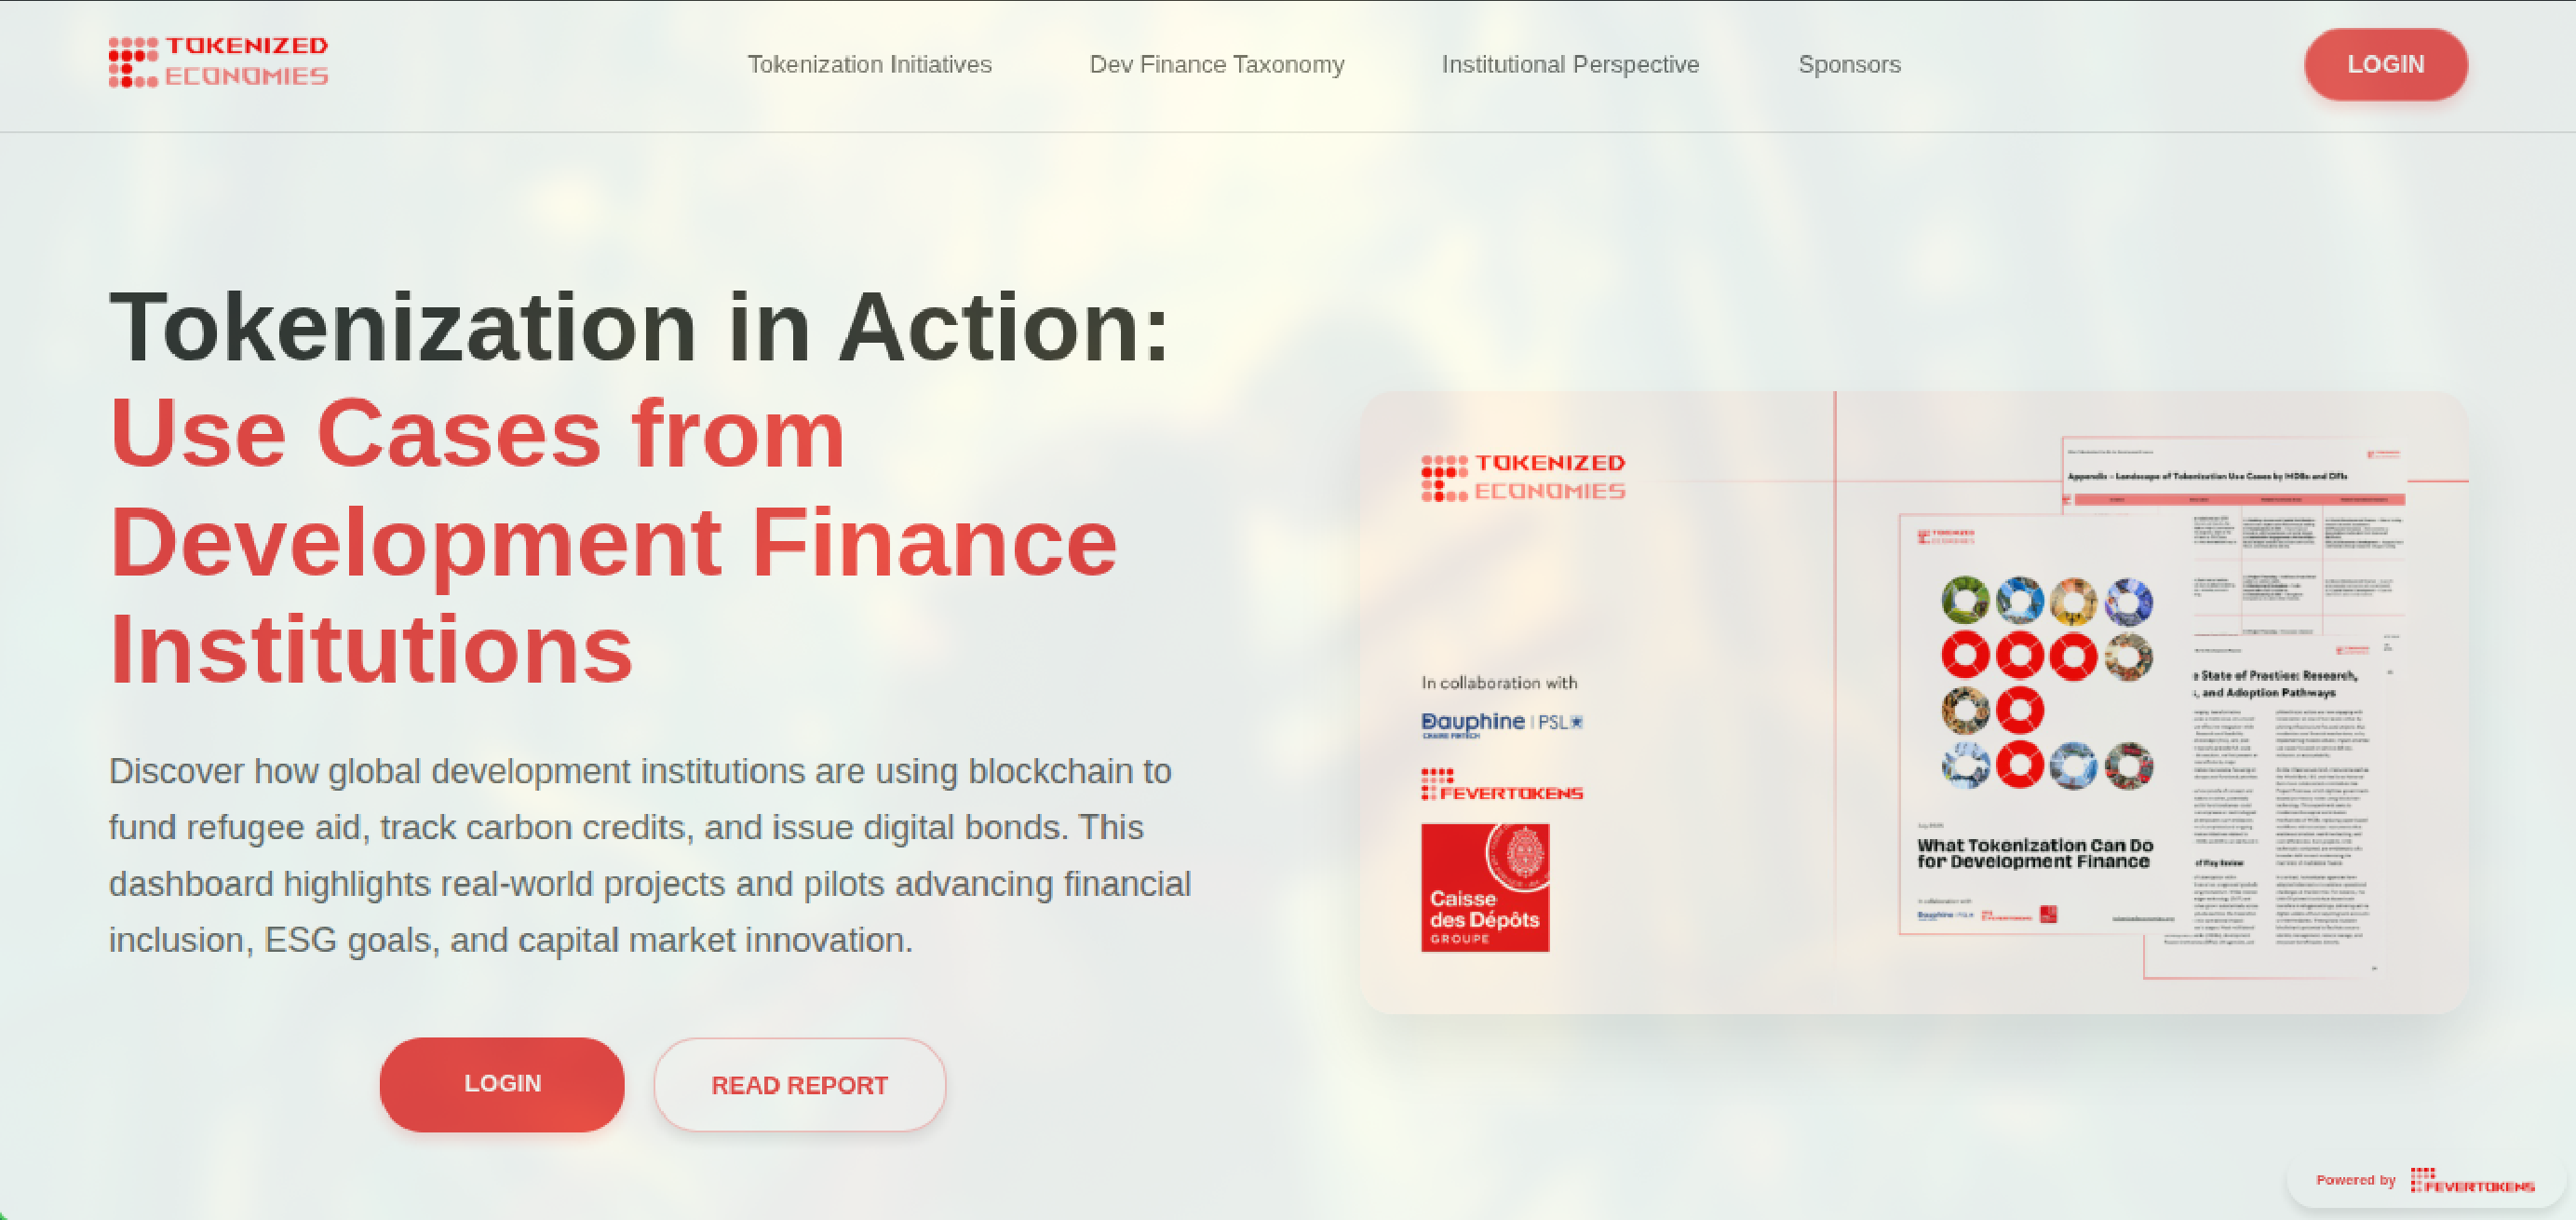
\includegraphics[width=0.85\textwidth]{figures/tei_landing.pdf}
    \caption{l'application TEI-TDFD.}
    \label{fig:tei_architecture}
\end{figure}
\vskip.25cm
Le projet \textbf{TEI-TDFD} (\textit{Tokenized Economies Institute – Tokenized Development Finance Dashboard}) s'inscrit dans le domaine de la \textbf{finance du développement}, qui regroupe l'ensemble des services financiers soutenant la croissance économique, en particulier dans les pays à revenu faible et intermédiaire. Les \textit{banques multilatérales de développement} (MDBs) et les \textit{institutions de financement du développement} (DFIs) constituent les acteurs principaux de ce secteur, en finançant des infrastructures essentielles et des projets sociaux. Toutefois, ce domaine se heurte aujourd'hui à des défis majeurs liés au manque de transparence, à la lourdeur des processus et à une gouvernance parfois inefficace.\\[2mm]
La \textbf{tokenisation}, qui consiste à représenter des actifs ou droits réels sous forme de jetons numériques sur des technologies de registre distribué (\textit{DLT}), apporte une réponse prometteuse à ces enjeux. Elle permet d'accroître la traçabilité, la participation et la liquidité des projets de financement, tout en réduisant les risques liés aux points de défaillance centralisés. Dans le contexte actuel, marqué par des tensions géopolitiques et des besoins de financement croissants, l'application de la blockchain et de la tokenisation ouvre de nouvelles perspectives pour atteindre les objectifs de développement global.\\[2mm]
C'est dans ce cadre que s'inscrit \textbf{TEI-TDFD}, conçu comme une \textbf{application Web interactive} destinée à \textit{centraliser, gérer et analyser des initiatives liées à la finance du développement}. L'application permet aux utilisateurs de :
\begin{itemize}
    \item Créer un compte et gérer leur organisation (en devenir propriétaire).
    \item Explorer toutes les initiatives publiques et interagir via likes et commentaires.
    \item Visualiser leurs domaines opérationnels et zones fonctionnelles.
    \item Créer de nouvelles initiatives avec visibilité publique ou interne à l'organisation.
    \item Gérer les utilisateurs et initiatives (propriétaire d'organisation et administrateurs).
\end{itemize}
Un rôle de \textbf{super administrateur} assure la vérification des organisations et la gouvernance générale de la plateforme. \\[2mm]

\subsection{Stack Technologique et Architecture}
L'application repose sur une architecture moderne, facilitant la modularité, le partage de code et la maintenance. Son \textbf{stack technologique} comprend :
\begin{itemize}
    \item \textbf{Frontend :} Next.js 15 avec App Router pour des interfaces réactives et performantes.
    \item \textbf{Base de données :} PostgreSQL avec Drizzle ORM pour une gestion fiable et typée des données.
    \item \textbf{Authentification :} Better Auth avec le plugin organisation pour la gestion sécurisée des utilisateurs et rôles.
    \item \textbf{Emailing :} Nodemailer avec SMTP pour notifications et vérifications.
    \item \textbf{Sécurité :} Rate limiting, protection DDoS, et en-têtes de sécurité.\\
\end{itemize}

\subsection{Structure du Code et Monorepo}
Le projet \textbf{TEI-TDFD} est organisé en \textbf{monorepo}, regroupant l'ensemble des applications et packages dans un seul dépôt pour faciliter la modularité, la maintenance et le partage de code. Cette architecture permet également une meilleure coordination entre les différentes équipes et composants du projet. \\[1mm]
La structure principale du dépôt est la suivante :
\vskip5cm
        \begin{verbatim}
        TEI-TDFD
        ├── apps
        │   └── ft-app
        │       ├── fonts
        │       ├── messages
        │       ├── public
        │       └── src
        │           ├── app
        │           ├── components
        │           ├── config
        │           ├── contexts
        │           ├── data
        │           ├── hooks
        │           ├── i18n
        │           ├── layouts
        │           ├── lib
        │           ├── scripts
        │           ├── server
        │           ├── types
        │           ├── utils
        │           └── validators
        └── packages
            ├── config-tailwind
            ├── config-typescript
            ├── database
            ├── ft-core
            ├── services
            ├── types
            └── utils
        \end{verbatim}
Travailler sur ce monorepo m'a permis de mieux comprendre :
\begin{itemize}
    \item L'organisation d'un projet full-stack complexe avec séparation claire entre \textbf{frontend}, \textbf{backend} et \textbf{packages partagés}.
    \item La structure modulaire et réutilisable des composants (\textit{components, hooks, utils, lib}) pour un développement efficace.
    \item L'intégration de la base de données via \textbf{Drizzle ORM} et la coordination entre les modules backend et frontend.
    \item La gestion des configurations et types partagés via les packages \textit{config-typescript}, \textit{config-tailwind}, \textit{types} et \textit{utils}, facilitant la maintenabilité et la cohérence du code.
\end{itemize}
Cette architecture monorepo a été un excellent apprentissage pratique pour la gestion de projets à grande échelle dans un environnement full-stack Web3 et cloud.

\subsection{Interface Utilisateur et Screenshots}
\begin{figure}[H]
    \centering
    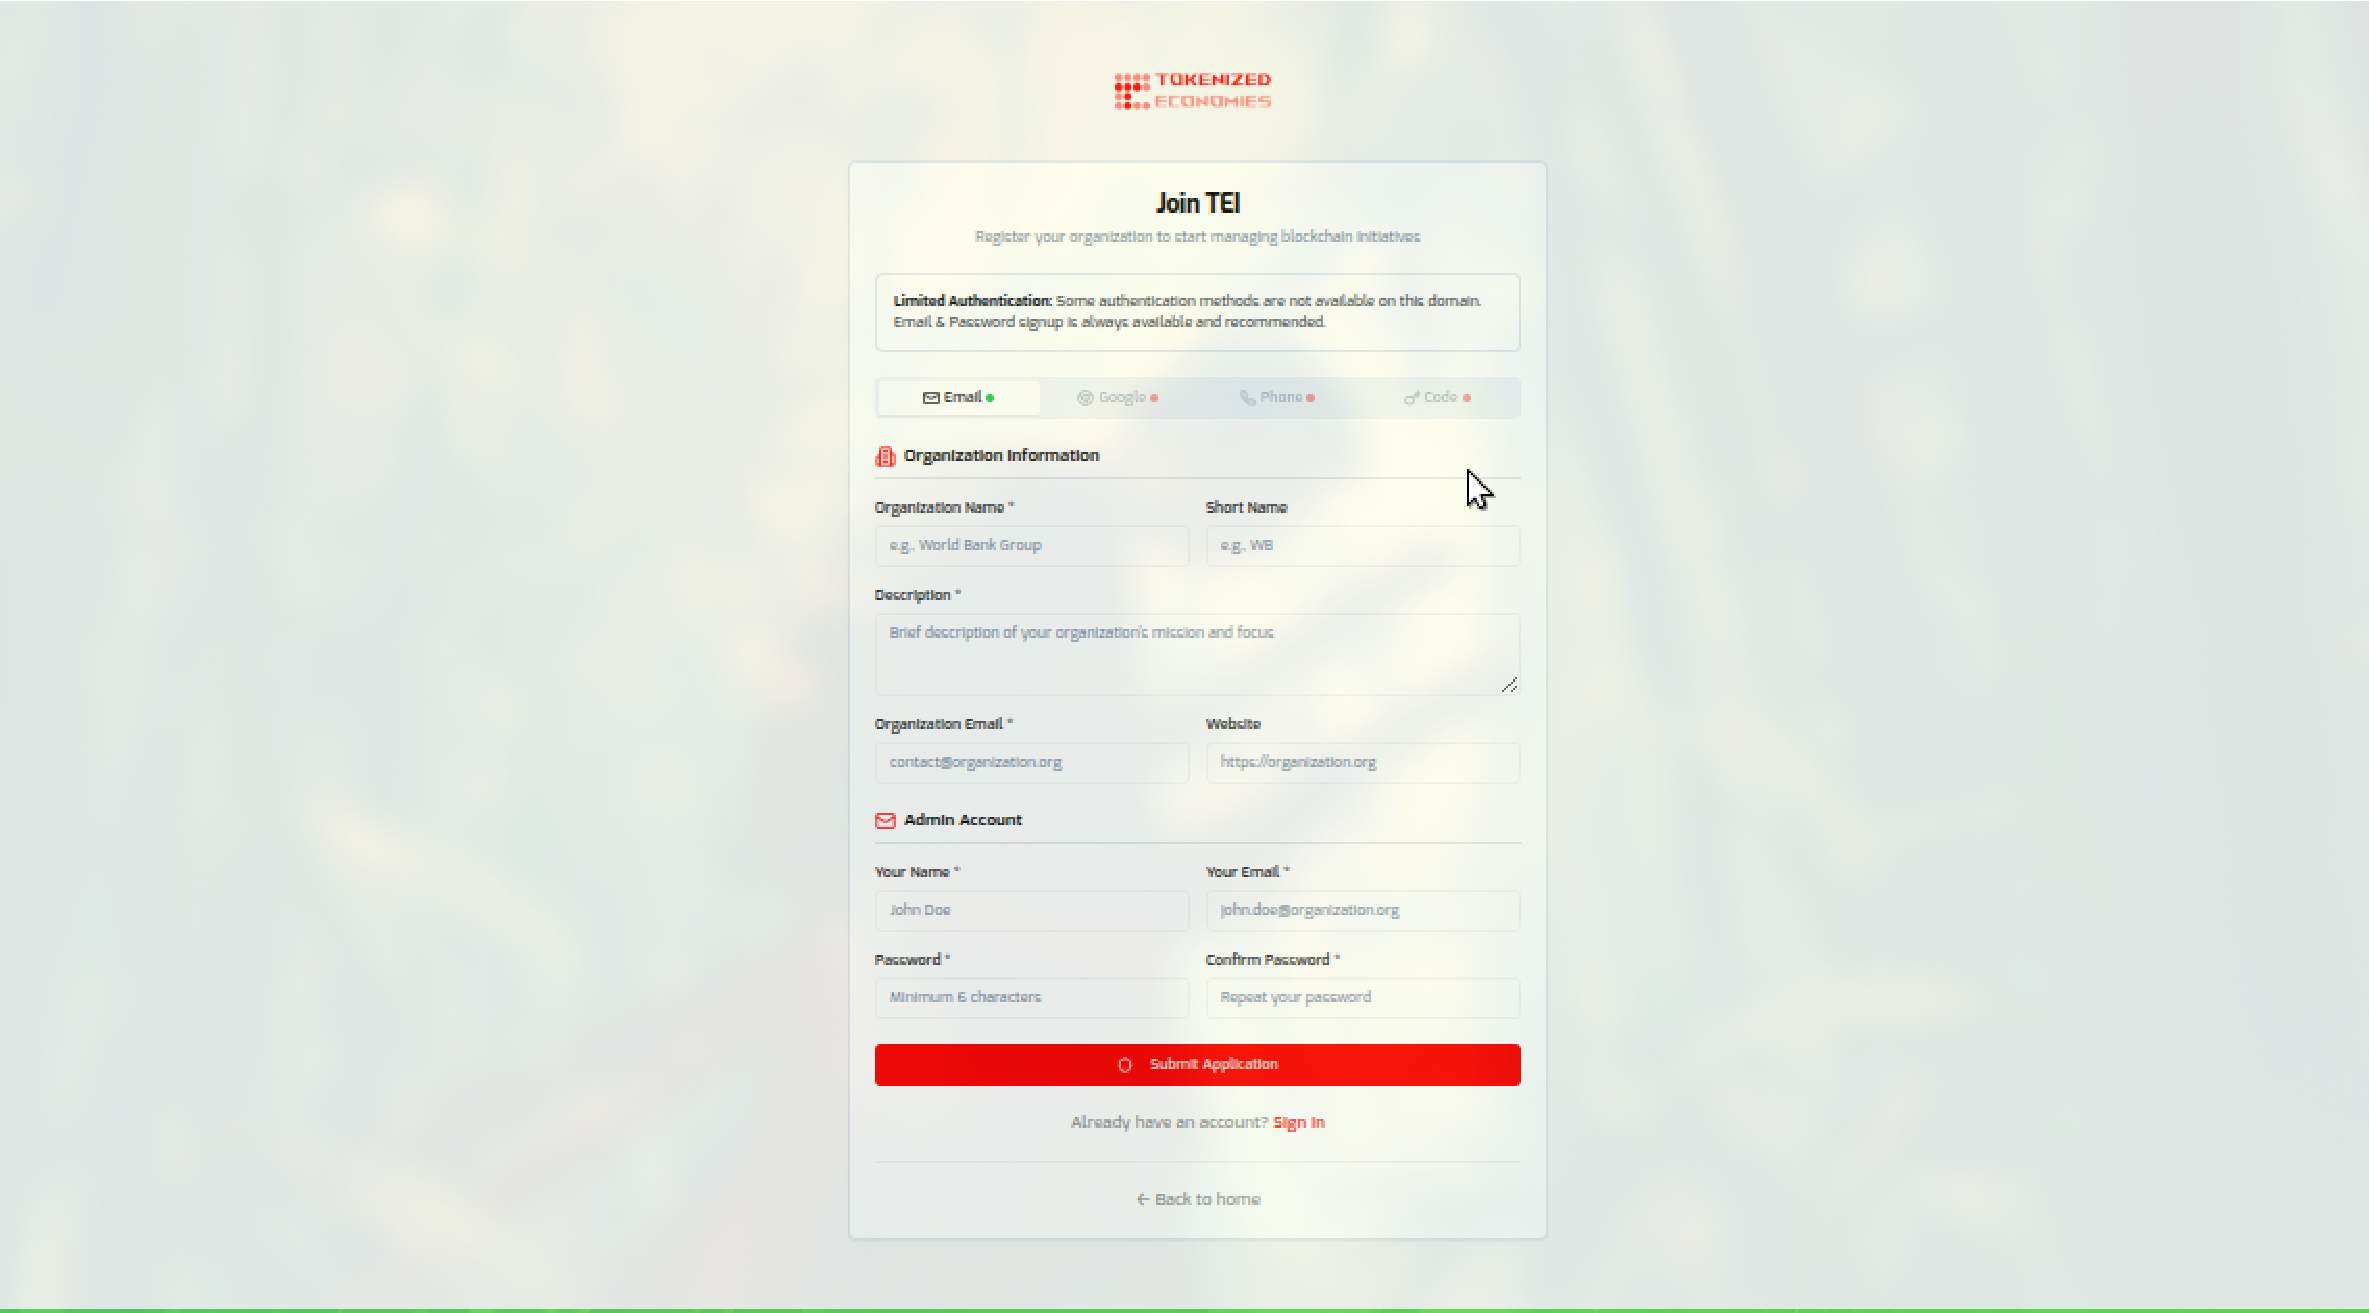
\includegraphics[width=0.7\textwidth]{figures/tei_signup.pdf}
    \caption{Page sign-up de TEI-TDFD.}
\end{figure}

\begin{figure}[H]
    \centering
    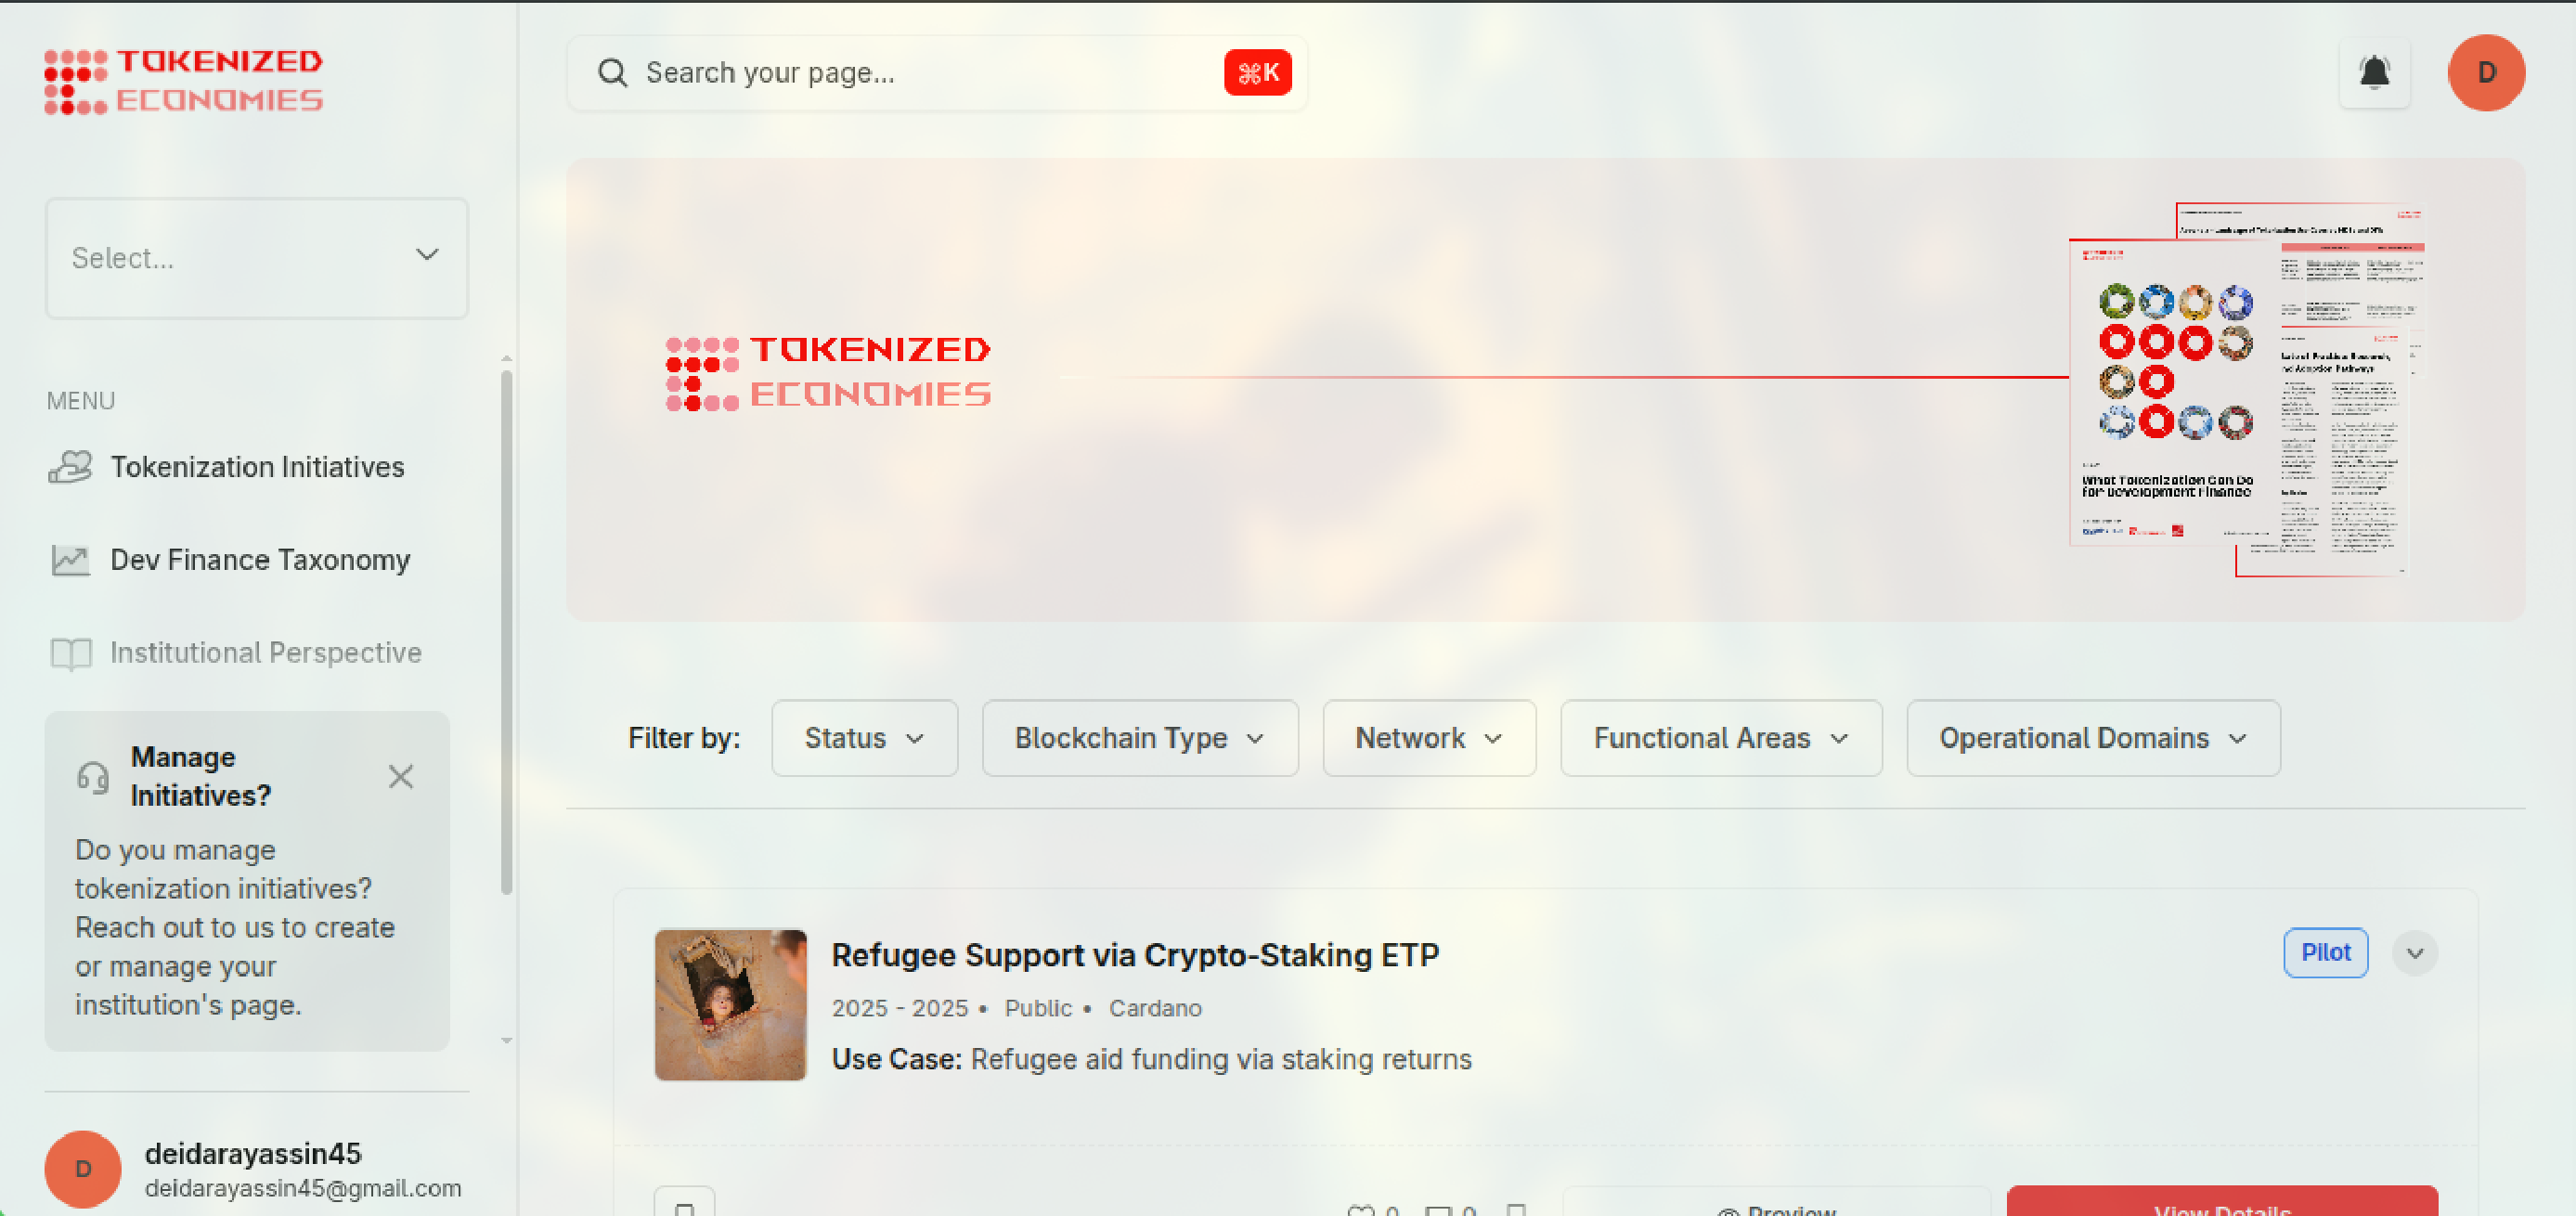
\includegraphics[width=0.7\textwidth]{figures/tei_initiatives.pdf}
    \caption{Page des initiatives publiques.}
\end{figure}

\begin{figure}[H]
    \centering
    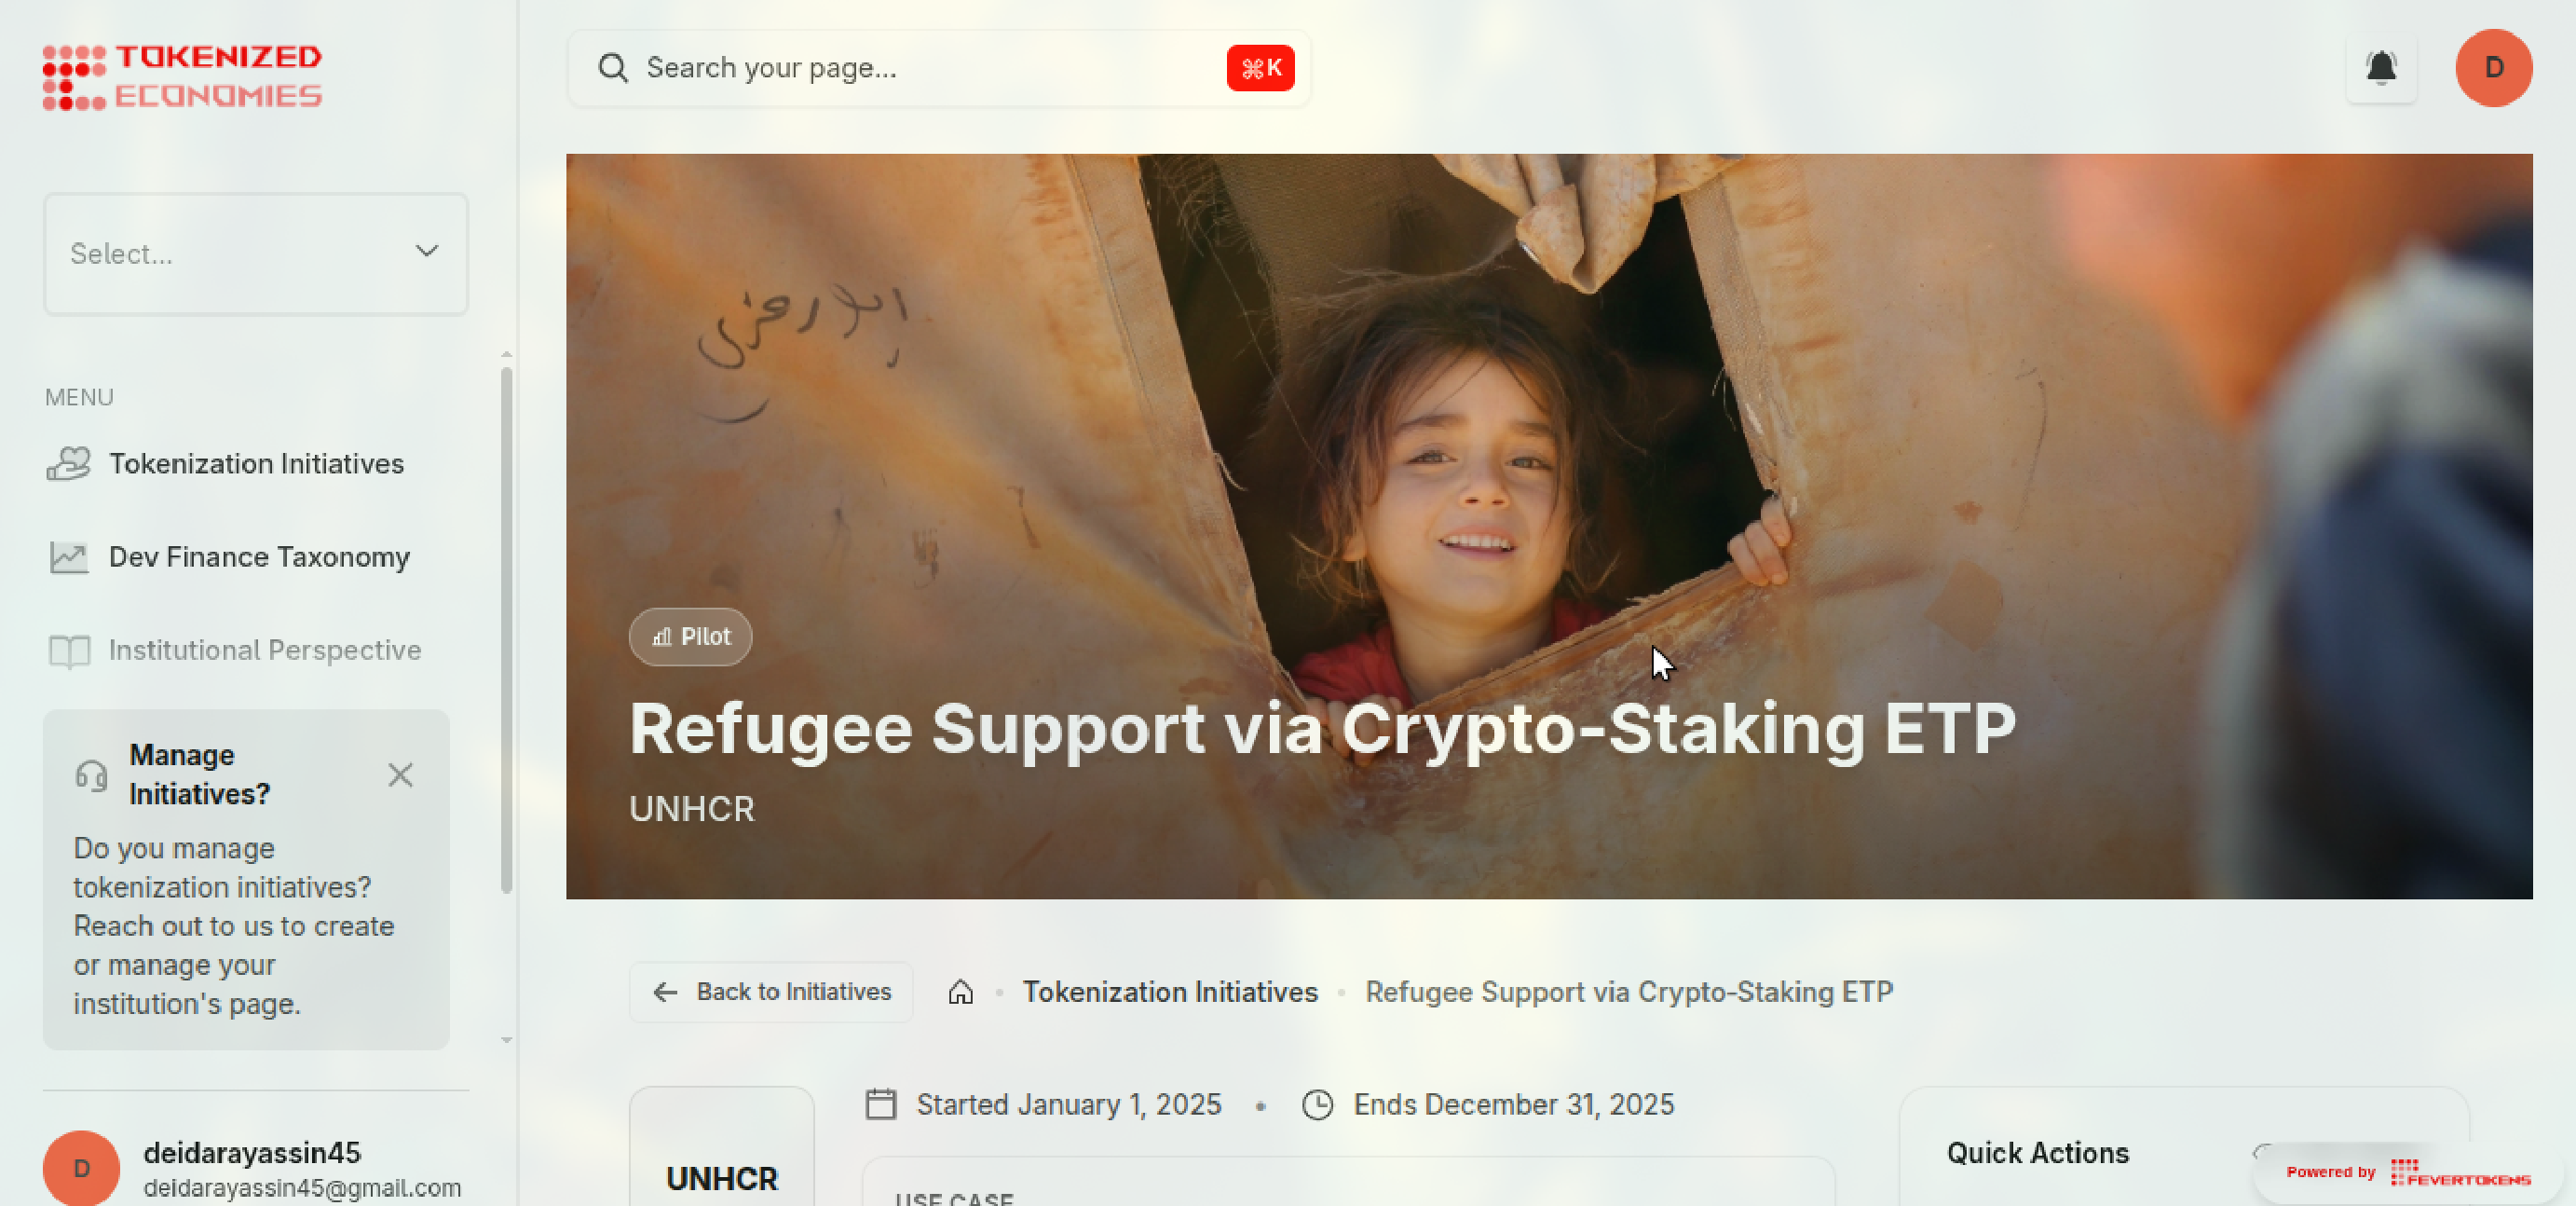
\includegraphics[width=0.7\textwidth]{figures/tei_initiative-detail-1.pdf}
    \caption{Page d'une initiative spécifique 1.}
\end{figure}

\begin{figure}[H]
    \centering
    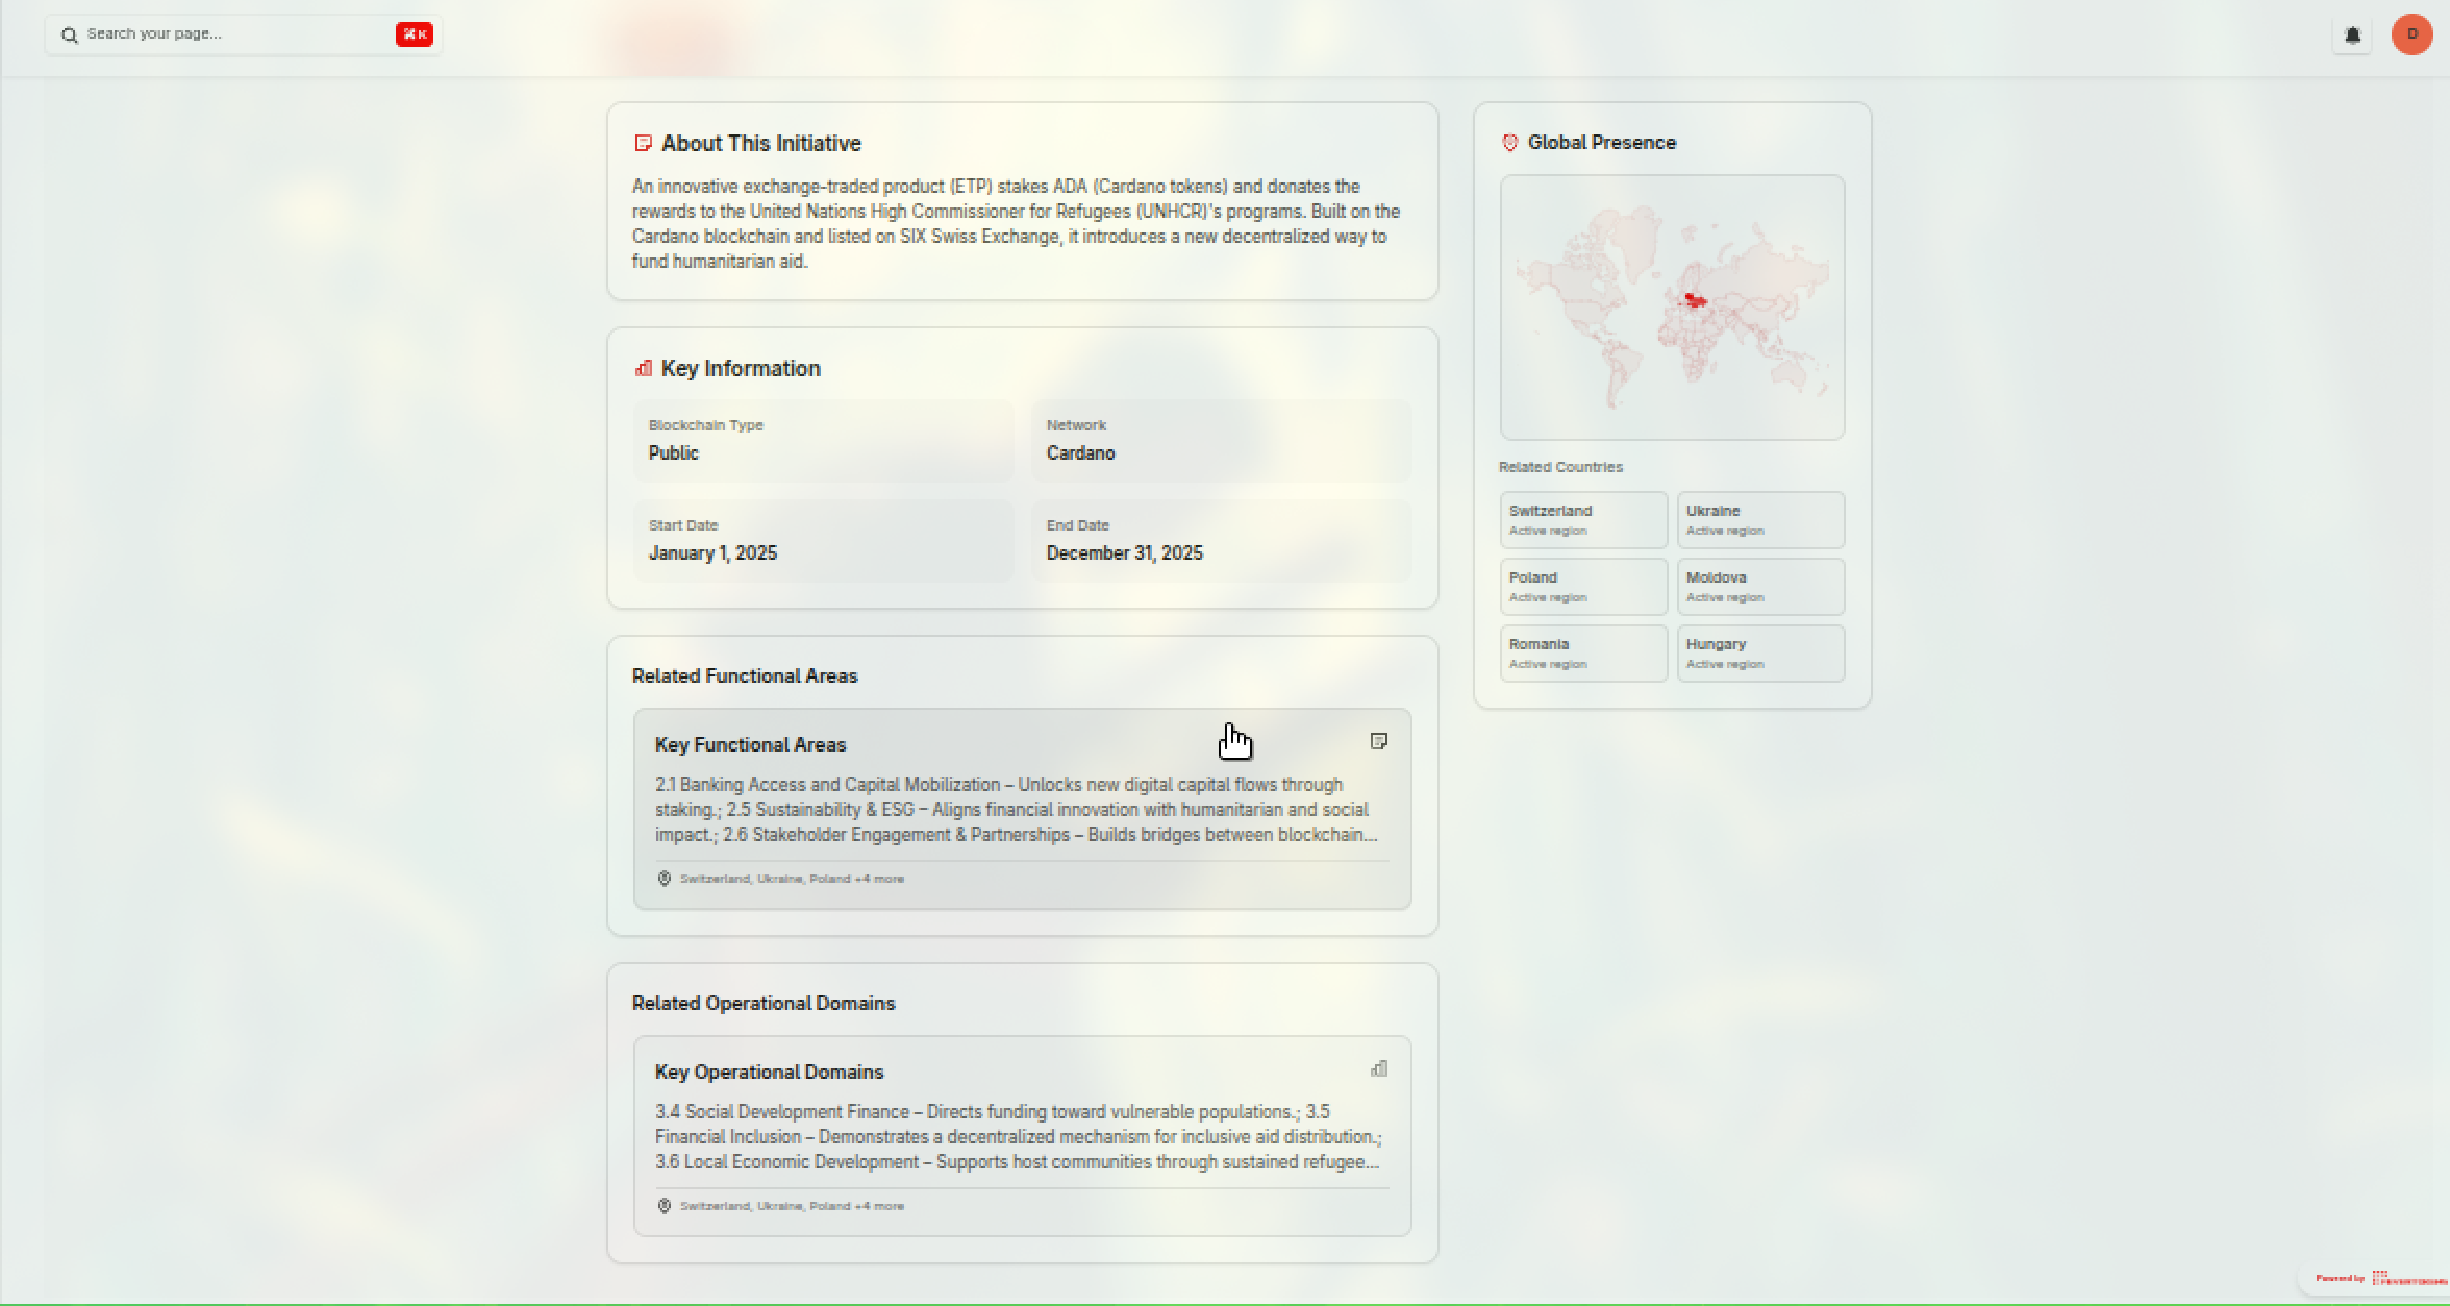
\includegraphics[width=0.7\textwidth]{figures/tei_initiative-detail-2.pdf}
    \caption{Page d'une initiative spécifique 2.}
\end{figure}
\vskip.5cm
\subsection{Rôle et Contributions}
Au cours de mon stage, j'ai pris en charge plusieurs tâches techniques majeures, chacune contribuant au développement et à l'amélioration de la plateforme TEI-TDFD. Ces tâches sont détaillées ci-dessous.\\

\leftskip1.5cm
\subsubsection{\uline{TEI-TDFD : Intégration de la base de données}}
\begin{figure}[H]
    \centering
    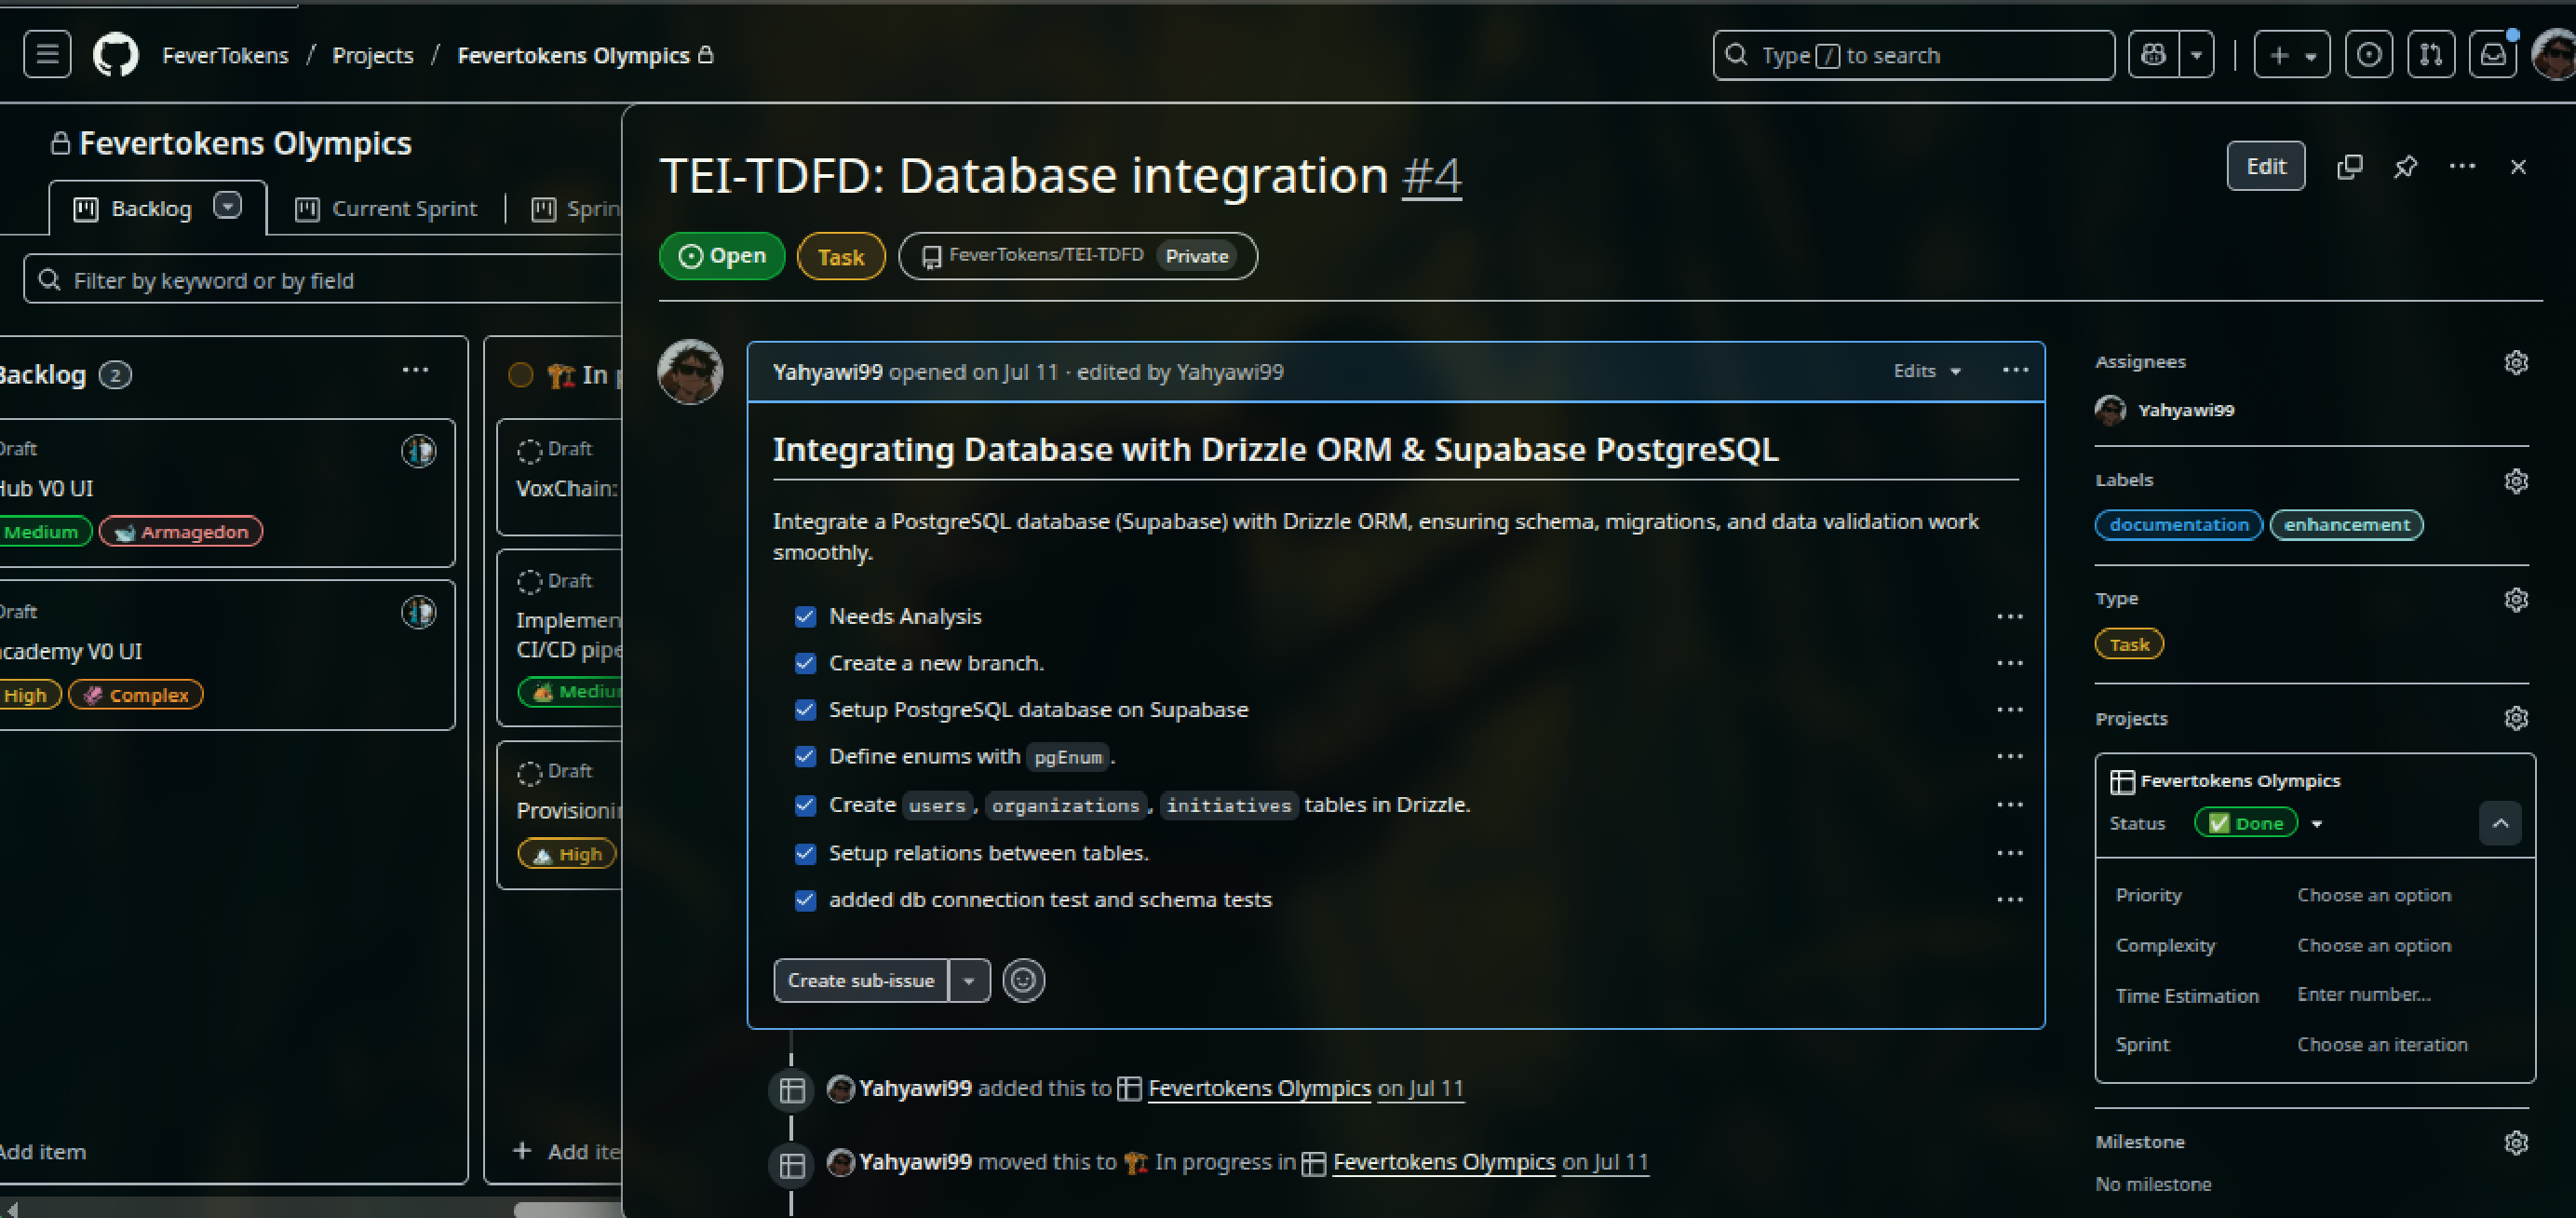
\includegraphics[width=0.7\textwidth]{figures/tei_taches_1.pdf}
    \caption{TEI-TDFD: Tache-1}
    \label{fig:TEI-TDFD_db}
\end{figure}
\vskip.25cm
\textbf{Objectif :} Intégrer une base de données PostgreSQL (Supabase) avec Drizzle ORM, afin d'assurer une gestion fiable des schémas, migrations et validations.\\
\textbf{Implémentation :}

\begin{itemize}
    \leftskip1.25cm
    \item Création d'une nouvelle branche dédiée.
    \item Mise en place de la base de données sur Supabase.
    \item Définition des \texttt{enums} avec \texttt{pgEnum}.
    \item Création des tables principales : \texttt{users}, \texttt{organizations}, \texttt{initiatives}.
    \item Mise en place des relations entre les tables.
    \item Ajout de tests de connexion et de validation du schéma.\\
\end{itemize}

\subsubsection{\uline{TEI-TDFD : Système de commentaires}}
\begin{figure}[H]
    \centering
    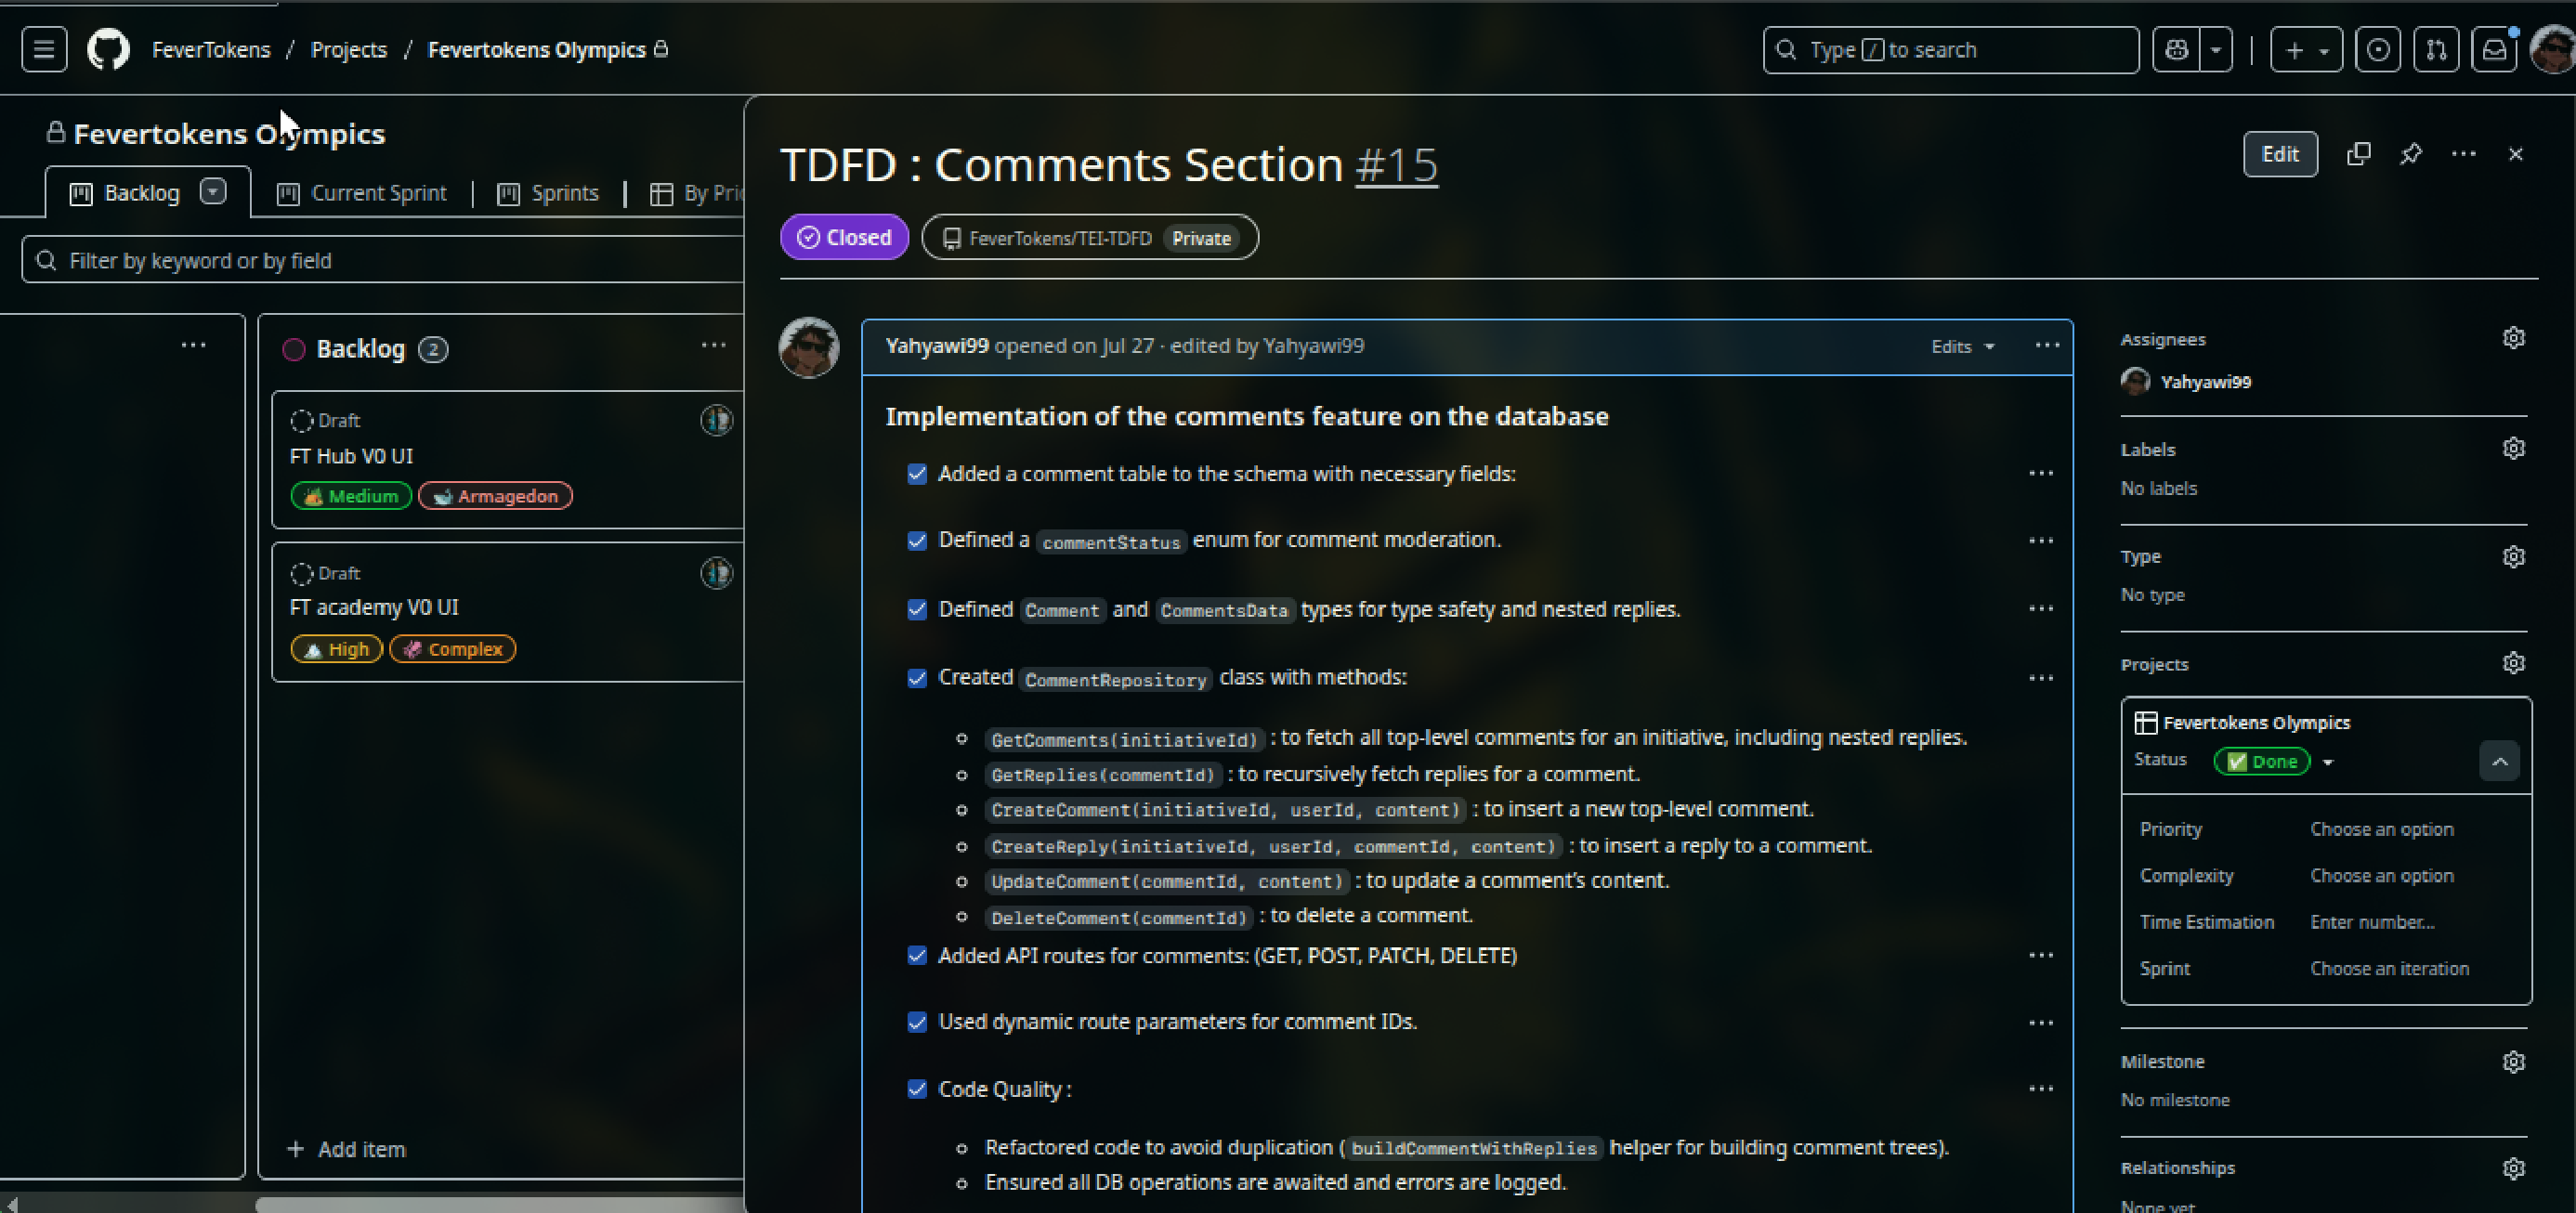
\includegraphics[width=0.7\textwidth]{figures/tei_taches_2.pdf}
    \caption{TEI-TDFD: Tache-2}
    \label{fig:TEI-TDFD_comments}
\end{figure}
\vskip.25cm
\textbf{Objectif :} Implémenter la fonctionnalité de commentaires pour permettre aux utilisateurs d'interagir sur les initiatives.\\
\textbf{Implémentation :}
\begin{itemize}
    \leftskip1.25cm
    \item Ajout de la table \texttt{comments} et d'un \texttt{enum} \texttt{commentStatus}.
    \item Définition des types \texttt{Comment} et \texttt{CommentsData} pour assurer la sécurité et la gestion des réponses imbriquées.
    \item Création d'une classe \texttt{CommentRepository} avec des méthodes : \texttt{GetComments}, \texttt{GetReplies}, \texttt{CreateComment}, \texttt{CreateReply}, \texttt{UpdateComment}, \texttt{DeleteComment}.
    \item Mise en place des routes API REST (GET, POST, PATCH, DELETE).
    \item Refactorisation avec un helper \texttt{buildCommentWithReplies} pour éviter la duplication.
\end{itemize}

% Screenshot GitHub Project + capture page "Initiative avec commentaires"

\subsubsection{\uline{TEI-TDFD : Gestion des initiatives}}
\begin{figure}[H]
    \centering
    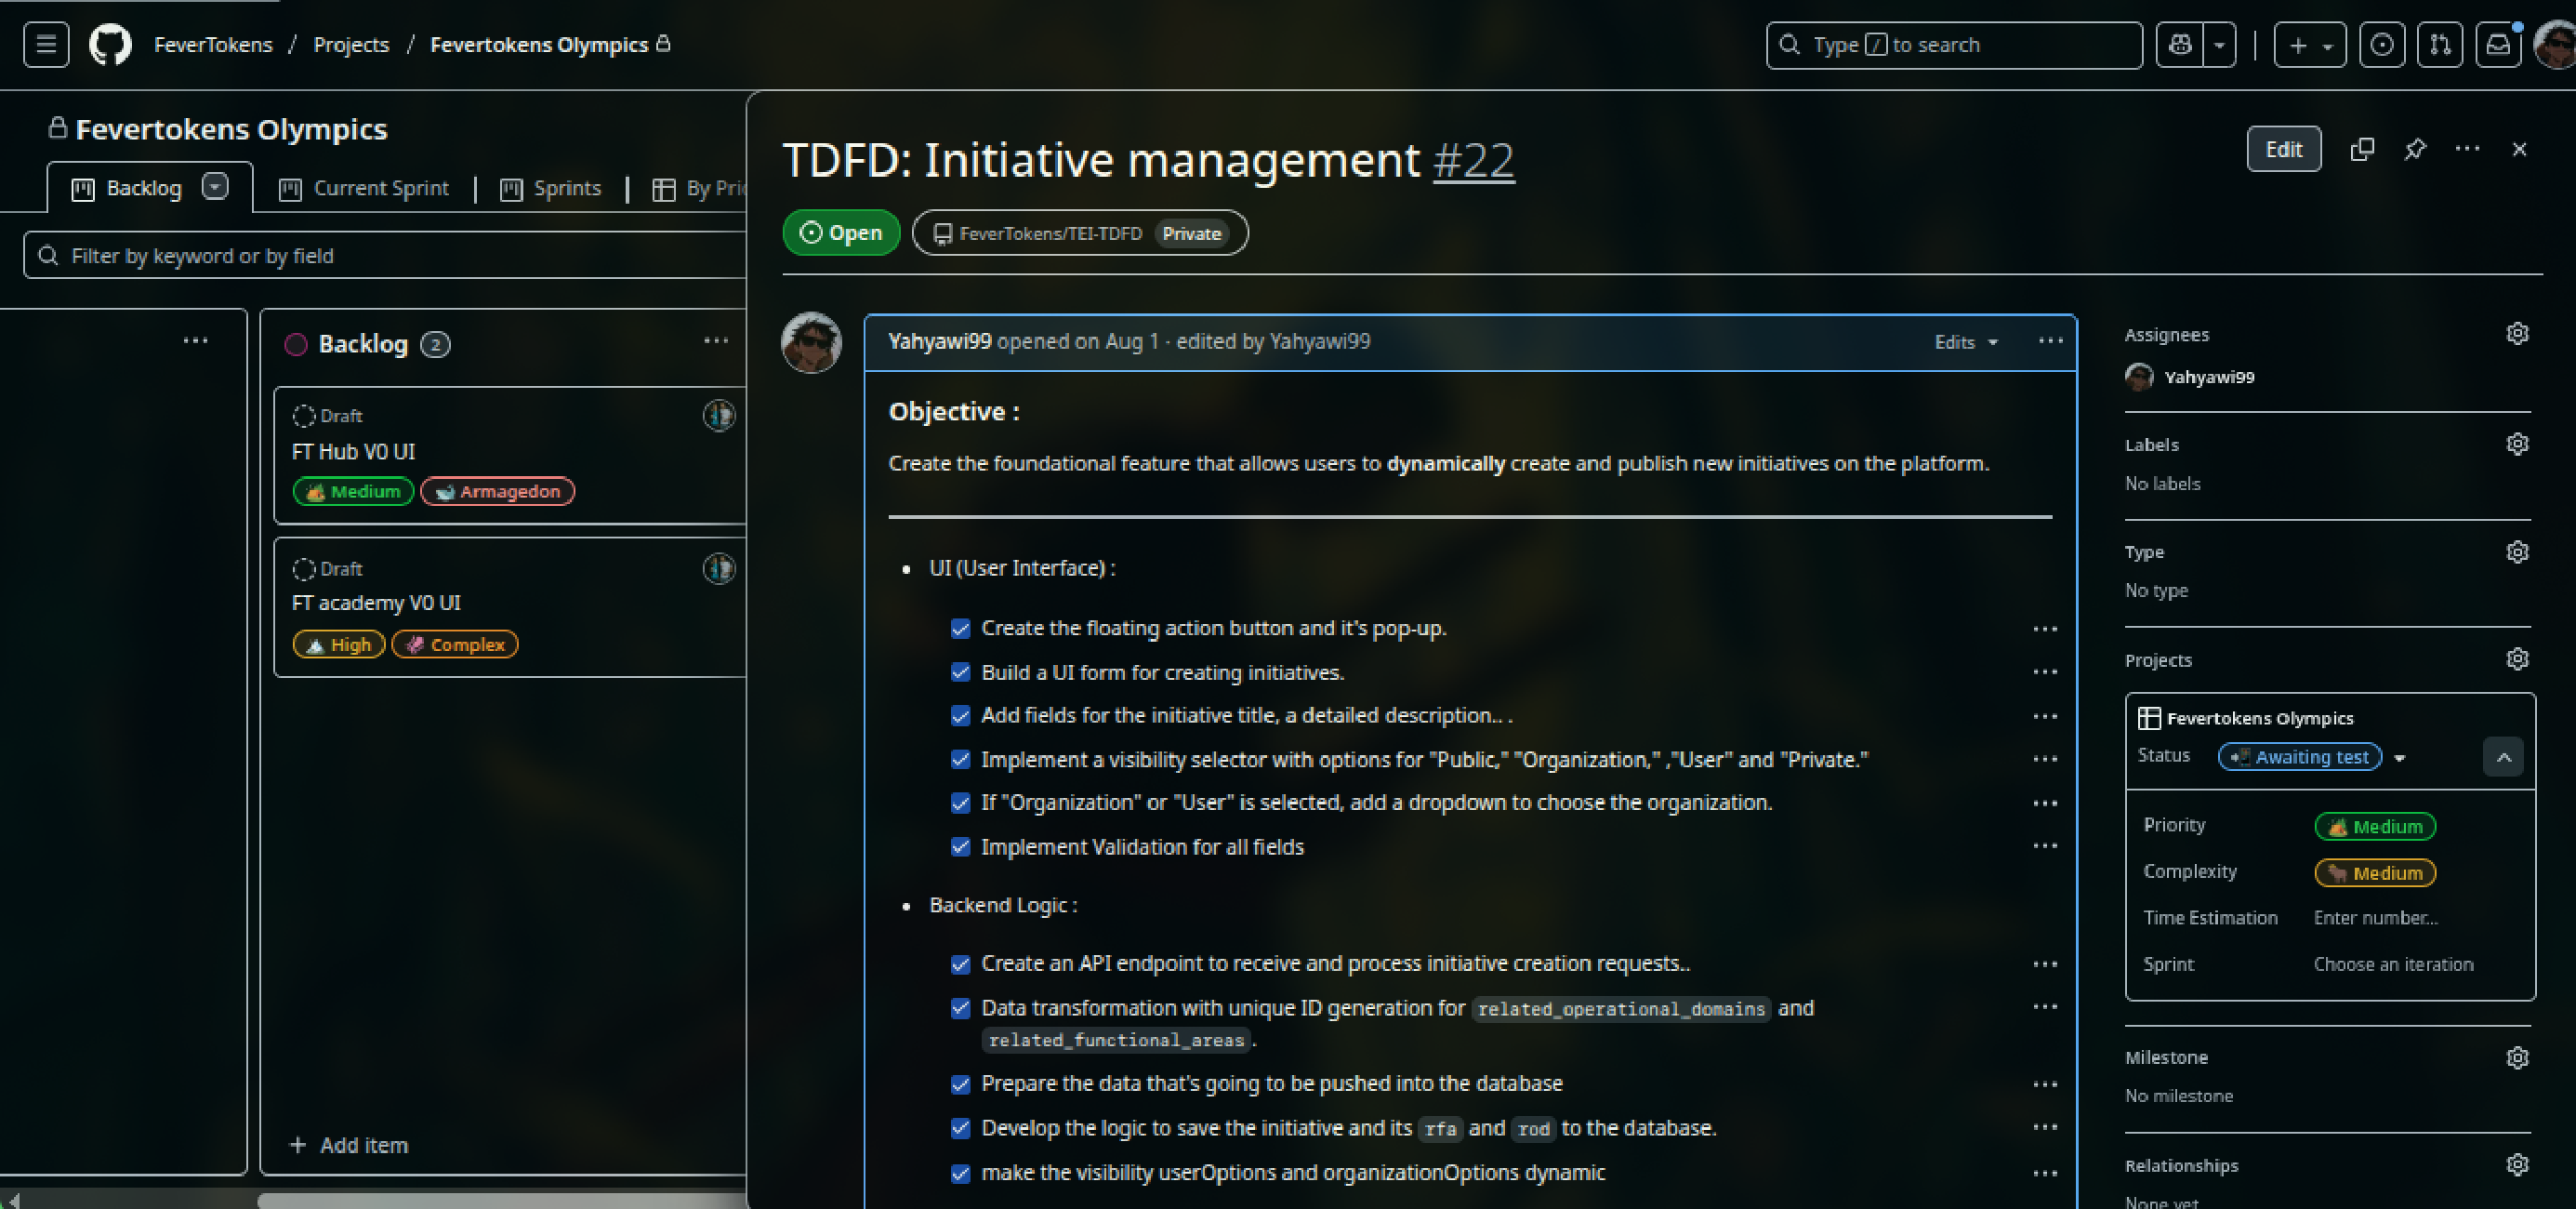
\includegraphics[width=0.7\textwidth]{figures/tei_taches_3.pdf}
    \caption{TEI-TDFD: Tache-3}
    \label{fig:TEI-TDFD_initiative}
\end{figure}
\vskip.25cm
\textbf{Objectif :} Permettre aux utilisateurs de créer et publier dynamiquement des initiatives.\\
\textbf{Implémentation :}
\begin{itemize}
    \leftskip1.25cm
    \item Création d'un bouton flottant et d'un formulaire de création d'initiative.
    \item Ajout de champs : titre, description détaillée, sélecteur de visibilité (\textit{Public}, \textit{Organisation}, \textit{Utilisateur}, \textit{Privé}).
    \item Génération dynamique des options selon l'organisation ou l'utilisateur.
    \item Validation de tous les champs avant soumission.
    \item Développement de l'API de création d'initiative (avec transformation des données et génération d'IDs uniques).
    \item Sauvegarde en base des initiatives avec leurs \texttt{related\_functional\_areas} et \\\texttt{related\_operational\_domains}.
\end{itemize}

% Screenshot GitHub Project + capture de l'UI "Create Initiative"

\subsubsection{\uline{TEI-TDFD : Documentation UI avec IA}}
\begin{figure}[H]
    \centering
    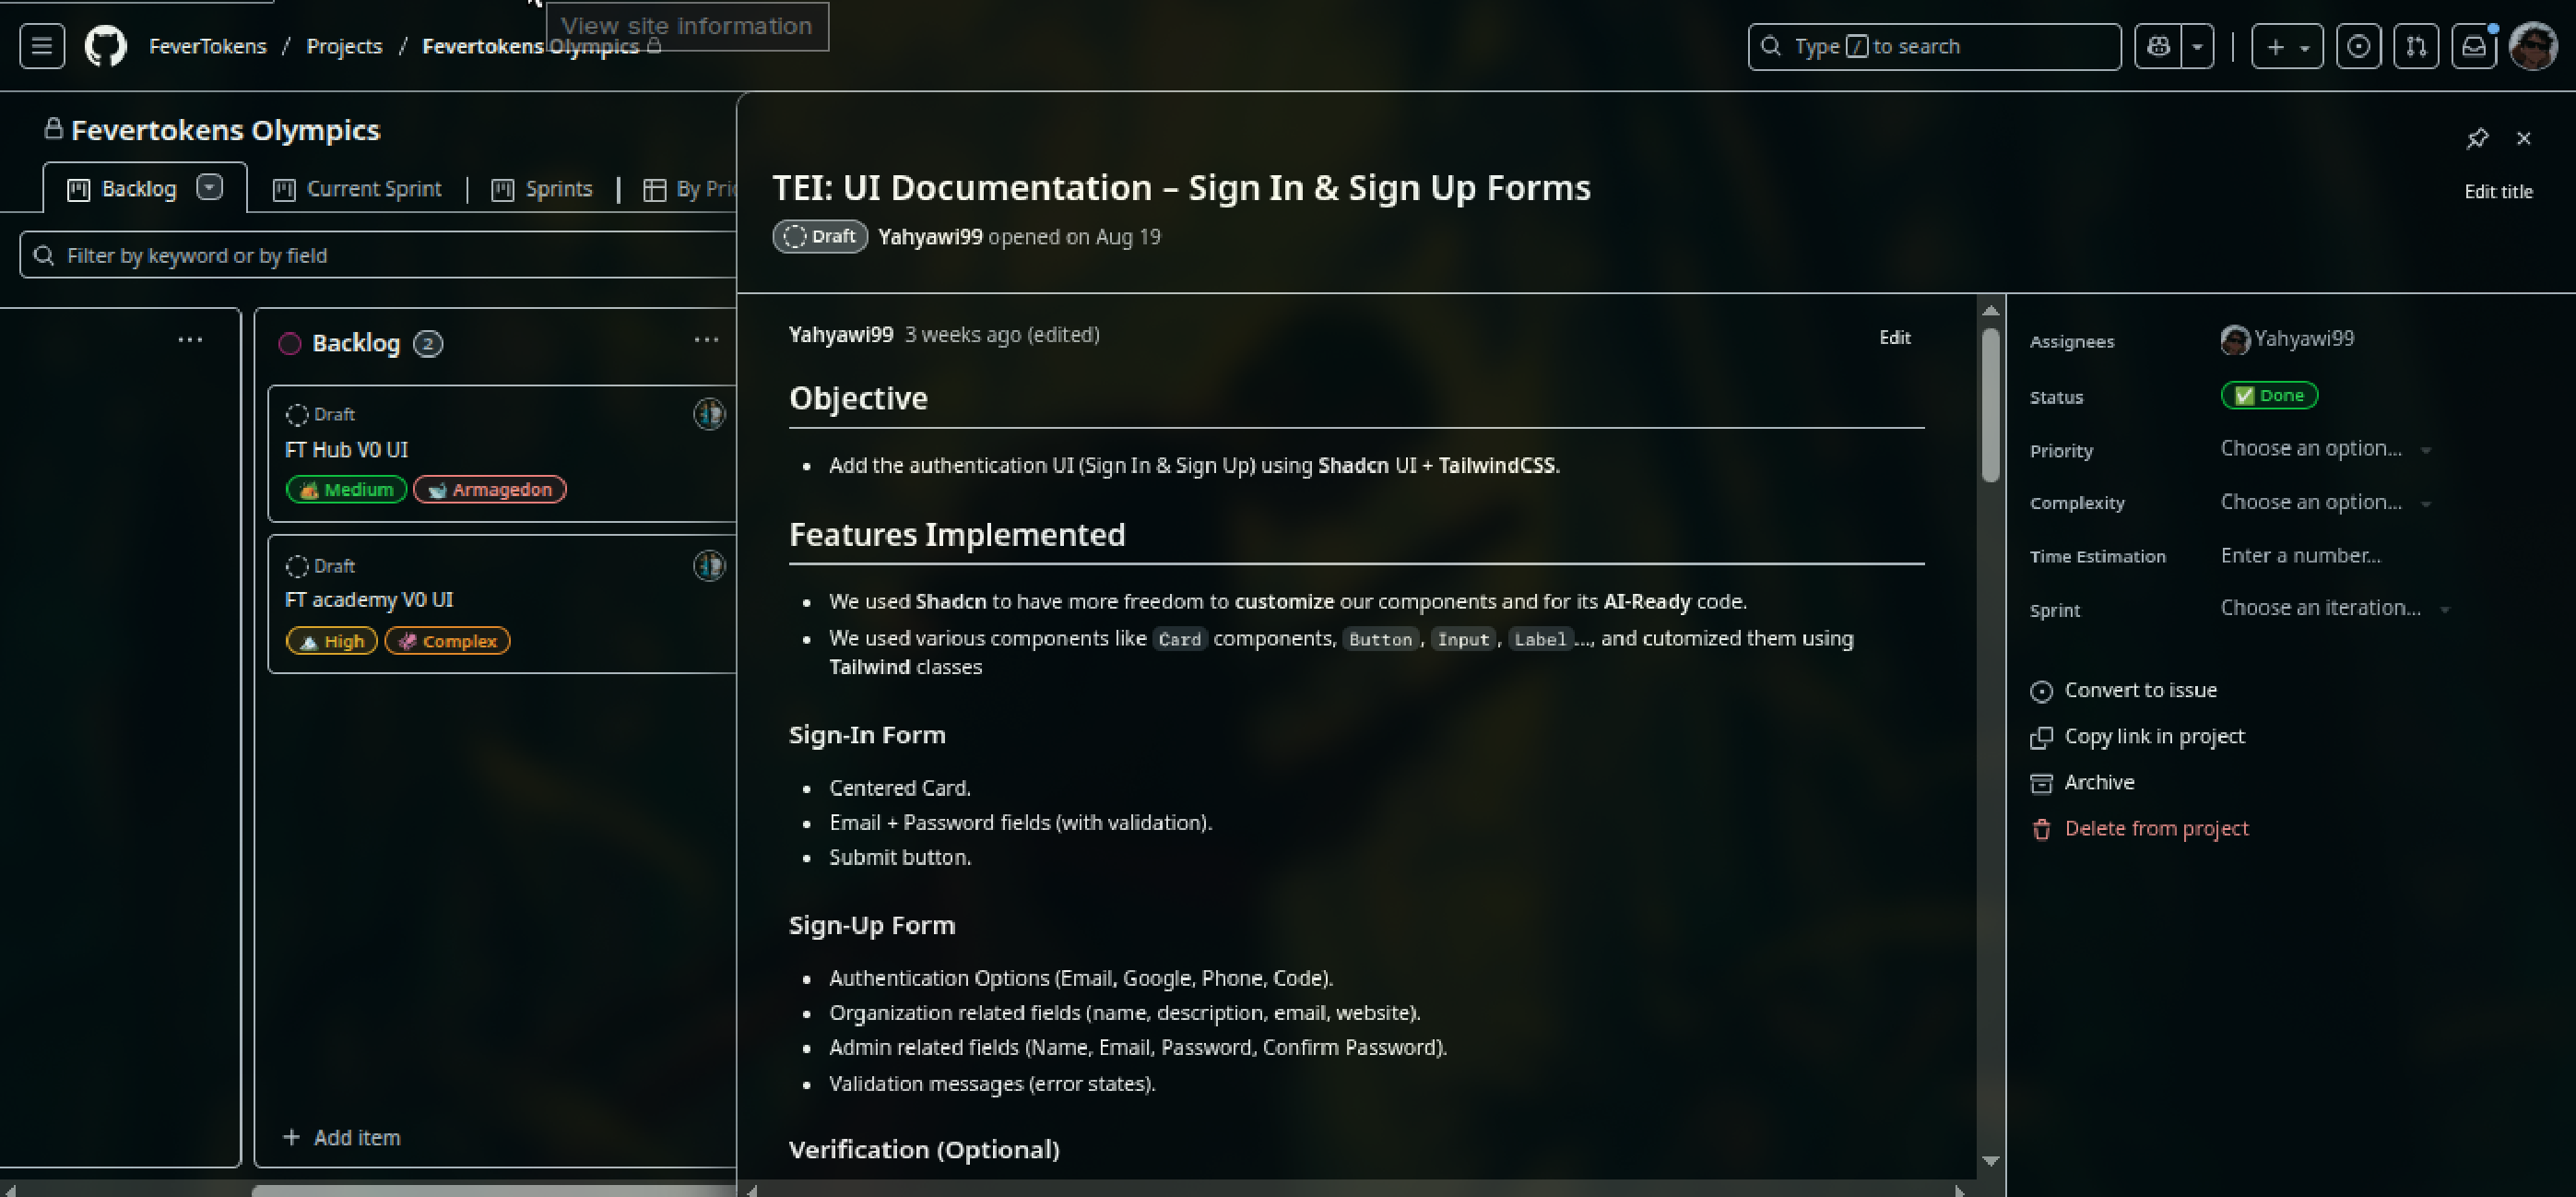
\includegraphics[width=0.7\textwidth]{figures/tei_taches_4.pdf}
    \caption{TEI-TDFD: Tache-4}
    \label{fig:TEI-TDFD_documentation}
\end{figure}
\vskip.25cm
\textbf{Objectif :} Générer une documentation guidée pour les formulaires d'inscription et de connexion.\\
\textbf{Implémentation :}
\begin{itemize}
    \leftskip1.25cm
    \item Utilisation d'outils d'IA (LLMs et Copilot) pour rédiger la documentation.
    \item Création de prompts spécifiques expliquant la conception des formulaires \textit{Sign In} et \textit{Sign Up}.
    \item Documentation structurée incluant étapes de design, bonnes pratiques et extraits de prompts utilisées.\\
\end{itemize}

\leftskip.75cm

\subsection{Compétences Acquises}
Au cours de ce stage, j'ai principalement consolidé mes compétences techniques et méthodologiques.\\
J'ai appris à manipuler efficacement une base de données PostgreSQL avec Drizzle ORM et Supabase, en mettant en place des schémas, des relations et des migrations.\\
Ce travail m'a permis de comprendre plus en profondeur la logique des bases de données relationnelles et leur intégration dans une application moderne.\\[2mm]
J'ai également amélioré ma maîtrise de la gestion de projet avec Git et GitHub, notamment à travers la création de branches, la gestion des pull requests et le suivi des tâches.\\
Ce stage m'a aussi permis de renforcer des compétences transversales, comme la communication en équipe, la résolution de problèmes techniques et l'organisation du travail dans un cadre collaboratif.\\
Ces apprentissages constituent une réelle valeur ajoutée pour mes futurs projets académiques et professionnels.\\

\leftskip0cm
\section{Présentations Régulières}
\leftskip0.75cm
Au cours du stage, des \textbf{présentations Régulières} étaient organisées pour approfondir des sujets techniques et partager les connaissances au sein de l'équipe. Chaque sujet était attribué par un superviseur et durait en moyenne \textbf{15 minutes}.\\[1mm]
Mon rôle variait selon les présentations : \textbf{assister} lorsque d'autres stagiaires présentaient, et \textbf{préparer et présenter} lorsque le sujet m'était attribué.\\[5mm]
Les principaux sujets abordés incluent :

\begin{itemize}
    \leftskip1cm
    \item \textbf{Prisma vs Drizzle} : comparaison des ORM et des choix d'implémentation pour la base de données.
        \begin{figure}[H]
            \centering
            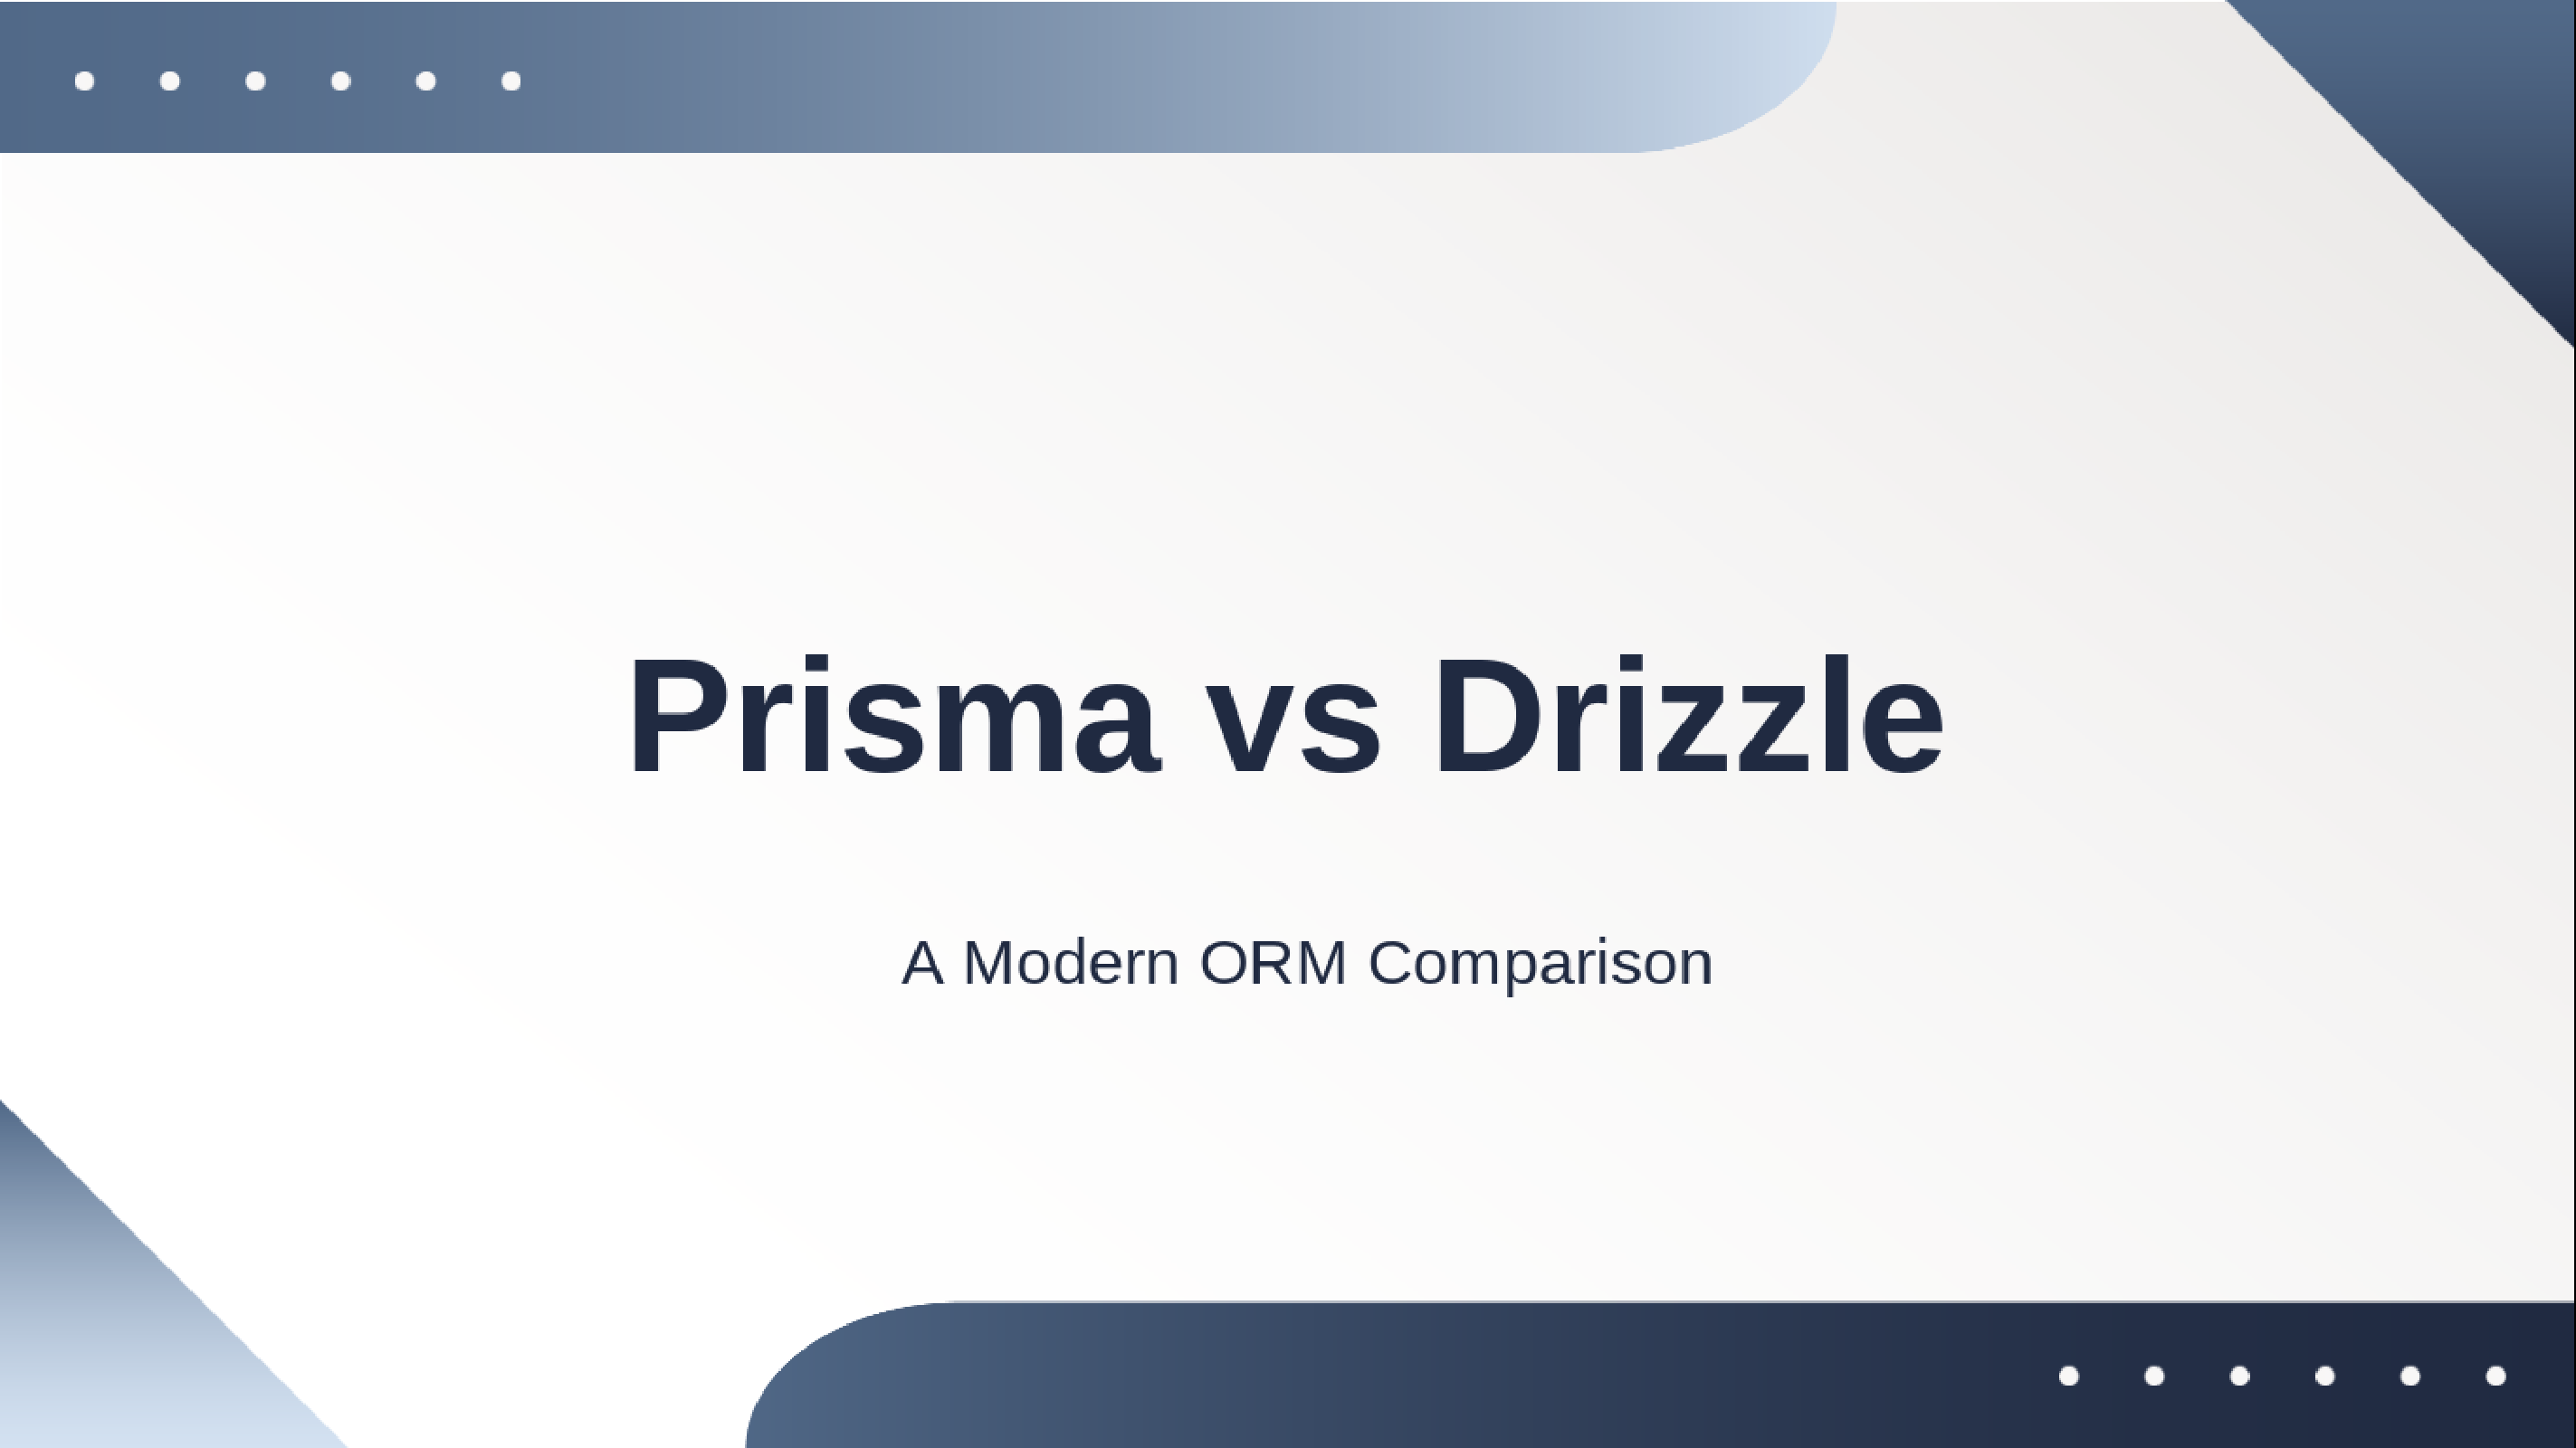
\includegraphics[width=.5\textwidth]{figures/presentation_1.pdf} 
            \caption{présentations Régulières: Prisma vs Drizzle.}
            \label{fig:weekly_presentations}
        \end{figure}
    \item \textbf{XML \& XSD} : compréhension des schémas et des structures de données utilisées dans le projet.
        \begin{figure}[H]
            \centering
            
\includegraphics[width=.5\textwidth]{figures/presentation_2.pdf} 
            \caption{présentations Régulières: XSD \& XML.}
            \label{fig:weekly_presentations}
        \end{figure}
    \item \textbf{Structure du code et bonnes pratiques TypeScript} : organisation des packages, typage strict et cohérence du code.
        \begin{figure}[H]
            \centering
            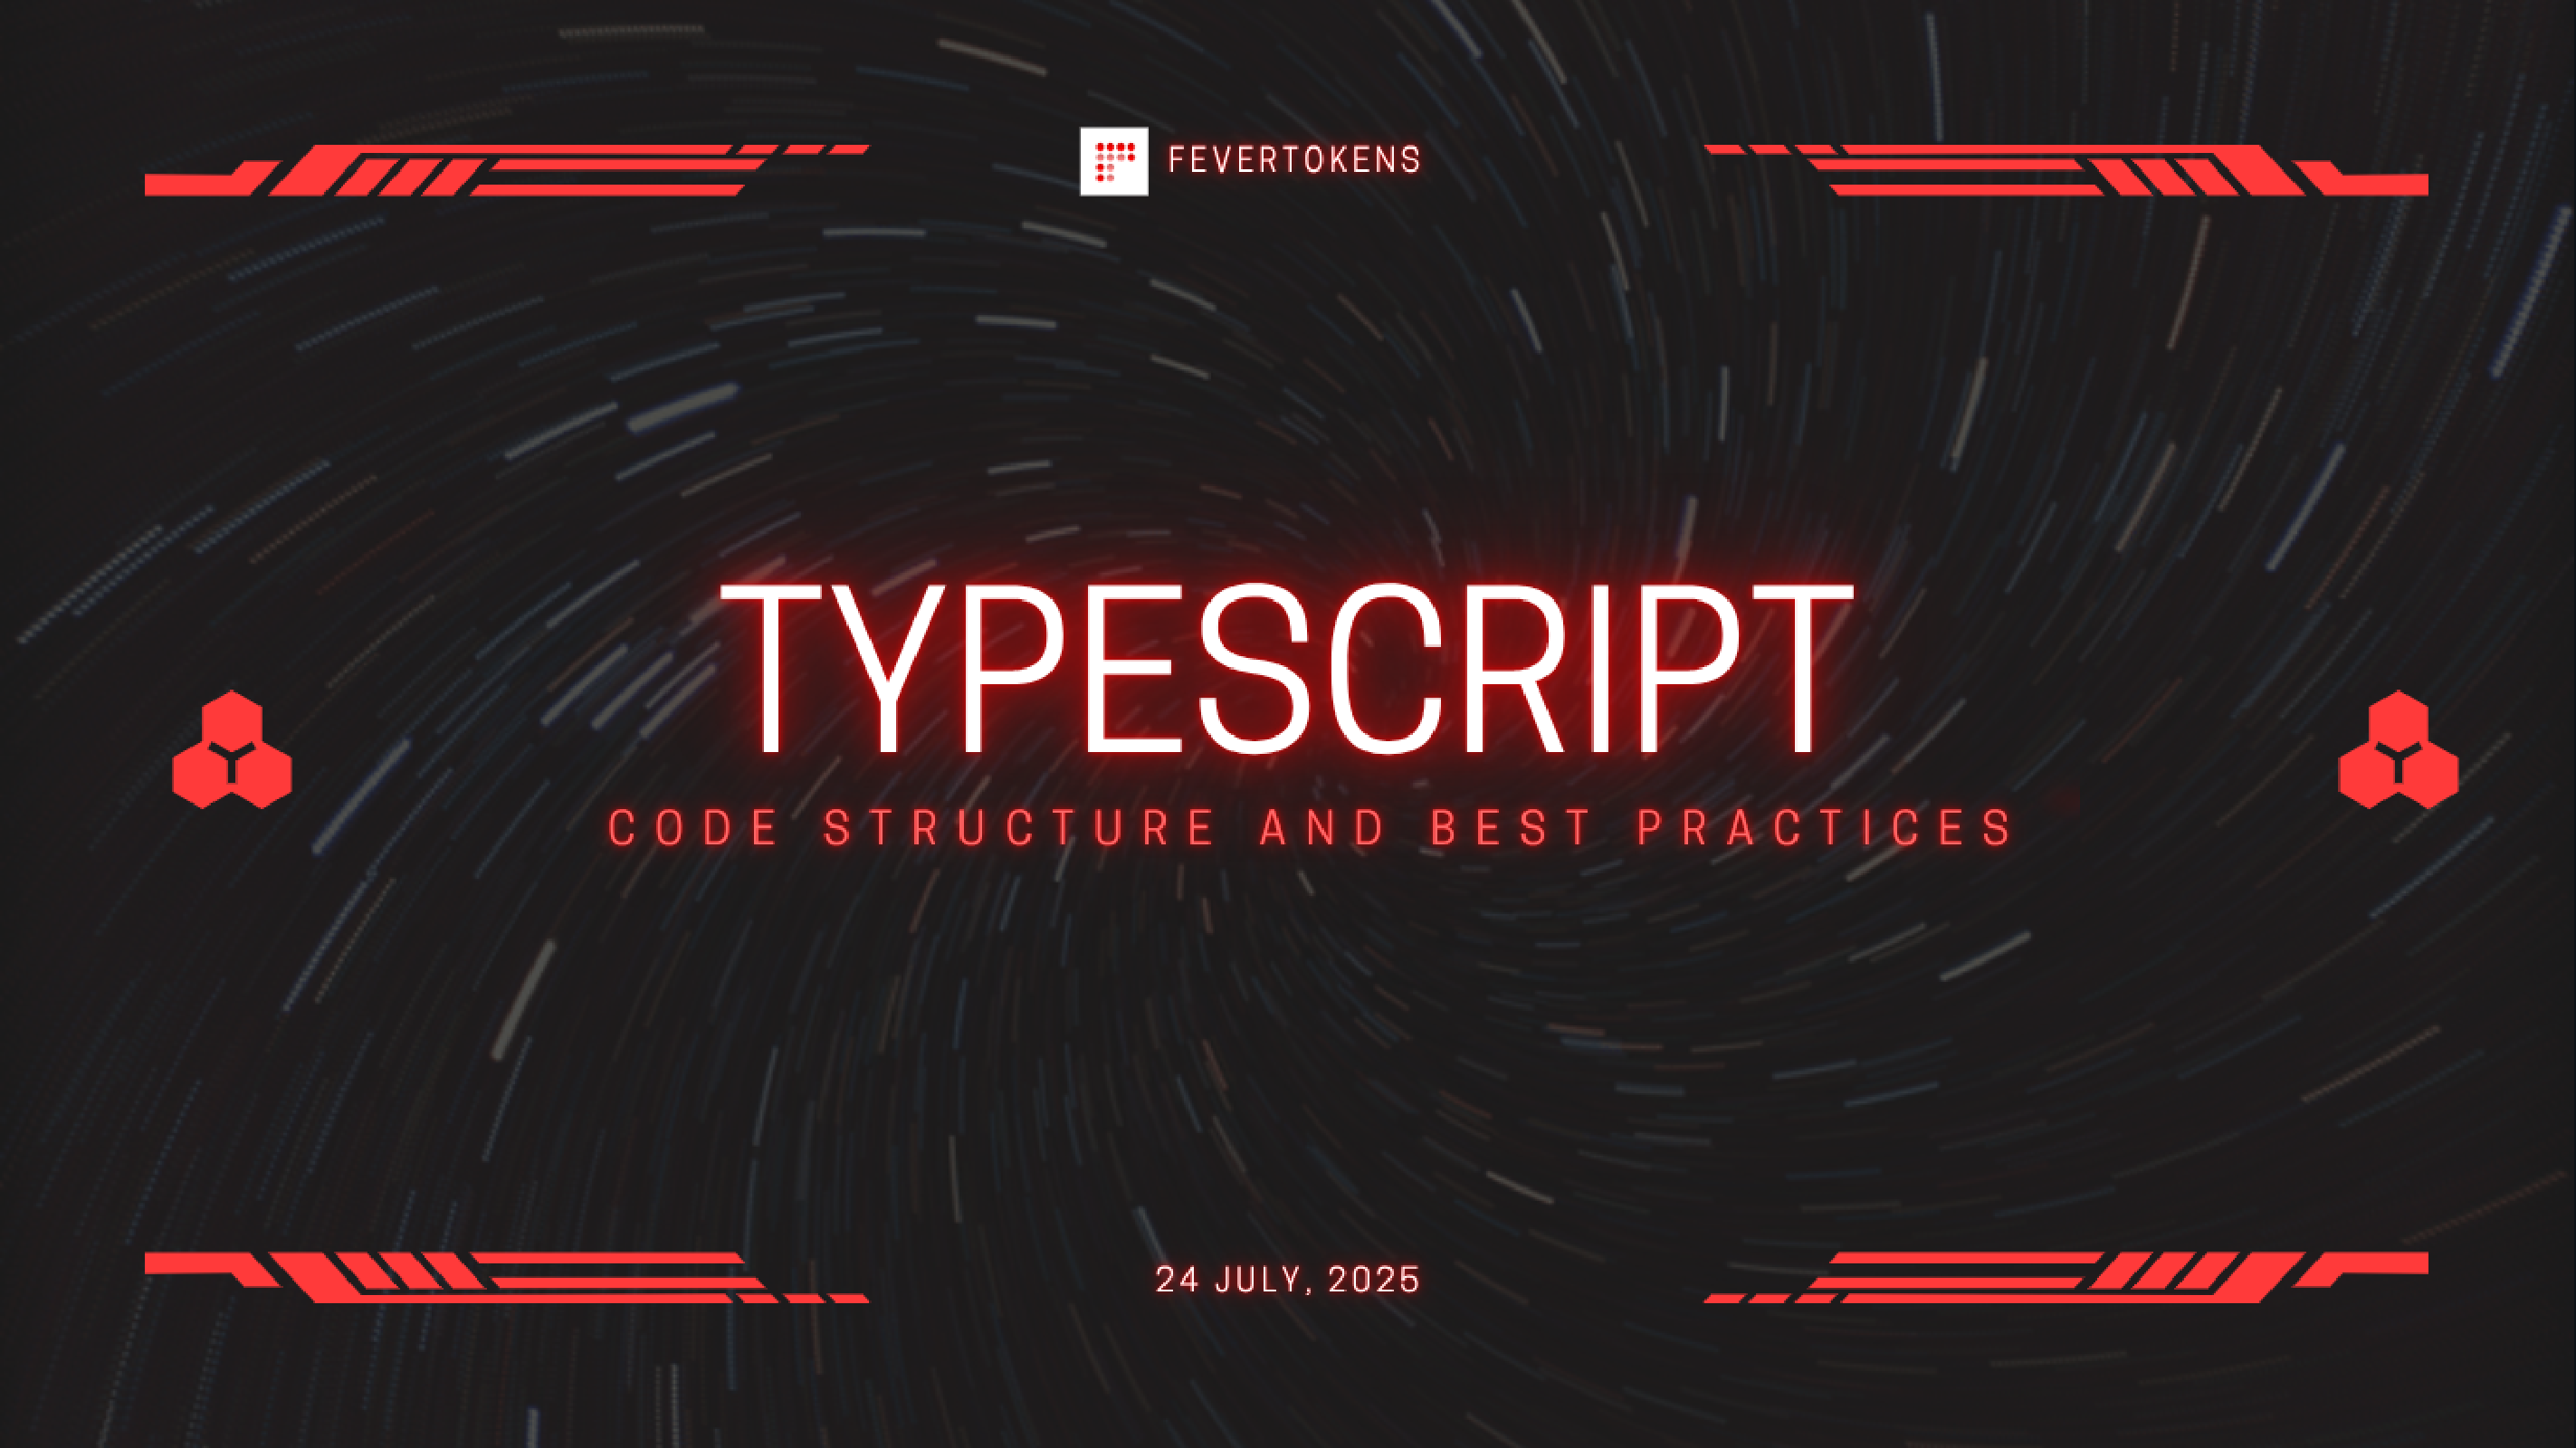
\includegraphics[width=.5\textwidth]{figures/presentation_3.pdf} 
            \caption{présentations Régulières: TypeScript.}
            \label{fig:weekly_presentations}
        \end{figure}
\end{itemize}
\vskip.5cm
\textbf{Résultats et apprentissages :} Ces présentations m'ont permis de communiquer plus librement, de surmonter ma peur de parler en public, et d'améliorer ma capacité à préparer et structurer une présentation technique claire et efficace.\\[1mm]

\leftskip0cm

\section{Conclusion}
Ce chapitre a permis de détailler les contributions principales et secondaires réalisées durant le stage, ainsi que les activités de suivi et de présentation qui ont favorisé à la fois l'avancement des projets et mon développement professionnel.
